\documentclass[a4paper,12pt,twoside]{book}
\usepackage[utf8]{inputenc}
\usepackage[english]{babel}
%\usepackage{fontspec}
%\setmainfont[
%  Ligatures=TeX,
%  Extension=.otf,
%  BoldFont=cmunbx,
%  ItalicFont=cmunti,
%  BoldItalicFont=cmunbi,
%  SlantedFont=cmunsl
%]{cmunrm}

%\usepackage{polyglossia}
%\setmainlanguage{spanish}

\usepackage[c5paper]{geometry}
%\geometry{inner=2.5cm,outer=2.5cm,bmargin=3.2cm}
%\usepackage[DIV=14,BCOR=2mm,headinclude=true,footinclude=false]{typearea}

%\usepackage{ulem} %Hace que \emph sea subrayar

%\usepackage[p,osf]{scholax}
%% T1 and textcomp are loaded by package. Change that here, if you want
%% load sans and typewriter packages here, if needed

\usepackage{ebgaramond}
%\usepackage[type1]{libertine} % Linux Libertine for zweispaltige Texte
%\usepackage{textcomp}% Required to get special symbols
\usepackage[scaled=.8]{DejaVuSansMono}% FiraMono Typewriter font
\usepackage{PTSansNarrow} 
%\gilliuscondensed
%\usepackage[sfdefault]{FiraSans}
%\usepackage{bm}% Extra bold faces
%\usepackage[lf]{carlito}

\usepackage{lettrine} %Capital letters at the beginning of a chapter
\usepackage[activate={true,nocompatibility},final,tracking=true,kerning=true,spacing=true,factor=1100,stretch=10,shrink=10]{microtype}
\SetTracking{encoding={*}, shape=sc}{-20} % versalitas menos separadas
% activate={true,nocompatibility} - activate protrusion and expansion
% final - enable microtype; use "draft" to disable
% tracking=true, kerning=true, spacing=true - activate these techniques
% factor=1100 - add 10% to the protrusion amount (default is 1000)
% stretch=10, shrink=10 - reduce stretchability/shrinkability (default is 20/20)

%\usepackage{array,multirow,booktabs,colortbl,chngcntr} % El último es para counterwithout;
\usepackage[strict]{changepage}
%\usepackage{caption}
%\captionsetup{format=plain,labelsep=newline,labelfont={small,sc},
%textfont={small,it},singlelinecheck=false}
\usepackage[Bjornstrup]{fncychap} % Para cabeceras de capítulos sofisticados:     Sonny,    Lenny,    Glenn,    Conny,    Rejne,    and Bjarne.

\usepackage{graphicx,wrapfig,booktabs,multicol,tabularx} % wallpaper: poner imágenes de fondo; wrapfigure: figuras a un lado del texto
%\graphicspath{{figures/}}
\usepackage{fancyhdr}
\usepackage{emptypage,pdfpages,fancybox} % Para que las páginas en blanco no tengan encabezado;
\usepackage{enumitem} %paralist: para compactenum, enumerate sin espacios
%\setlist[itemize]{nosep} %Espacio entre items en itemize
\usepackage[hyperref]{xcolor}
\usepackage[hidelinks]{hyperref}
\usepackage{xurl}

%\usepackage{minipage}

%\usepackage{quotchap} %Encabezados de capítulos
\usepackage{syntonly,verbatim}
%\syntaxonly

\usepackage{setspace,xspace} % xspace: Da \xspace para no tener que poner {} después de los comandos; pdflscape: páginas en horizontal;

\newenvironment{quotex}{\begin{quote}\small}{\end{quote}}
\newenvironment{quotationx}{\begin{quotation}\small}{\end{quotation}}


\begin{document}

% Por alguna razón, los marginados se creaban al revés. Así los corrijo. Feo, pero eficaz:
\let\tmp\oddsidemargin
\let\oddsidemargin\evensidemargin
\let\evensidemargin\tmp
\reversemarginpar

%\setcounter{secnumdepth}{4} % Para que llegue a numerar hasta las subsubsecciones;
%\renewcommand{\heavyrulewidth}{0.14em} % Grosor de las líneas extremas de las tablas;
%\renewcommand\thempfootnote{\alpha{mpfootnote}} % Símbolo de notas dentro de minipage
%\let\oldcaptionof\captionof
%\renewcommand{\captionof}[2]{\oldcaptionof{#1}{\newline \textit{#2} }}
%\renewcommand{\tablename}{Tabla}
%\counterwithout{figure}{chapter}
%\counterwithout{table}{chapter} % Así la numeración es 1, 2, 3... y no 1.1, 1.2... y no reinicia la num. en cada capítulo;

%\providecommand{\ggl}{\guillemotleft}
%\providecommand{\ggr}{\guillemotright\xspace}
\providecommand{\flright}[1]{\begin{flushright}#1\end{flushright}}
\providecommand{\flrightit}[1]{\begin{flushright}\itshape #1\end{flushright}}
%\renewcommand\UrlFont\sffamily
\urlstyle{tt}

\pagestyle{fancy}
\renewcommand{\sectionmark}[1]{\markright{#1}}
\renewcommand{\chaptermark}[1]{\markboth{#1}{}}

%Portada:
%\includepdf{00Portada}

\frontmatter
%
%\onehalfspacing
%\pagenumbering{Roman} %gobble es como empty

%\include{preindice}

%\fancyhf{}
%\fancyhead[LE]{\small \textbf{\thepage}$\quad$ Índice general}
%\fancyhead[RO]{\small Índice general $\quad$\textbf{\thepage}}
%\clearpage
\tableofcontents

%\doublespacing
\mainmatter

\fancyhf{}
\fancyhead[LE]{\small \thepage$\quad${\scshape\chaptername{} \thechapter}: \nouppercase{\itshape\leftmark}}
\fancyhead[RO]{\small \textsc{Section }\thesection{}: \nouppercase{\itshape\rightmark} $\quad$\upshape\thepage}
%\cfoot{\bfseries\thepage}

\pagenumbering{arabic}

%\onehalfspacing

% introductorios

\chapter{Introduction}

\chapter{Traditional psychology}
\section{Metaphysics and Philosophy}

Because we write about topics such as being, religion, knowledge, history and the like — topics philosophers like to deal with — some readers of Gornahoor have the mistaken impression that we are also philosophers. Hence, they presume we are defending a particular philosophico-religious system, or trying to promote one; then they desire to engage in debate, for their own unfathomable purposes. Philosophy in our time involves speculative theories about the nature of the world and mind or else a tedious logical analysis of words. This is far from our task. Readers wishing to discuss topics are obliged to read the entire blog, or at least related material, prior to drawing any conclusions.

As we pointed out in Metaphysical Positivism\footnote{\url{https://www.gornahoor.net/?p=1189}}, we regard metaphysics as an exact science analogous to physics.

\begin{description}
\item[Physics ]

The science of the natural, or external, world 

\item[Metaphysics ]

the science of the states of the inner world 

\end{description}
When someone denies the possibility of such metaphysical knowledge, they are like the bishops who denied the existence of Jupiter's moons discovered by Galileo. In the latter case, the solution is simple: look through the telescope. Analogously, in the former case, the solution lies in meditation or other spiritual exercises that will unveil the inner world. The obstacle is, however, that in metaphysics, ``to know is to be". That means that, in order to know a particular inner state, one's very being much change to be in that state. Few are willing to go through the trouble; perhaps it is not even an option for many.

Such a change in being is not required in order to look through the telescope, a task that is readily accomplished by anyone. Therefore, physics is universal, democratic and egalitarian. Metaphysics is necessarily just the opposite.

We relate this to the trichotomous structure of man\footnote{\url{https://www.gornahoor.net/?p=1029}} in Table~\ref{tab:trichotomous}.

\begin{table}[h]\small\centering
\begin{tabular}{ll}\toprule
Spirit &
Non-formal manifestation\\
Soul &
Subtle manifestation\\
Body &
Gross manifestation\\\bottomrule
\end{tabular}
\caption{The trichotomous structure of man}
\label{tab:trichotomous}
\end{table}
The body is part of gross manifestation, or nature. It is subject to the laws of physics. We may not be accustomed to regarding our soul life as part of manifestation, but it consists of our thought, desires, moods, feelings, daydreams, fantasies, likes, dislikes and so on. It is part of our human state. Physics is the science of gross manifestation, metaphysics of subtle manifestation or higher states. Hence, just as the physicist is detached when he studies the movements of the planets, so also must the metaphysician be when he observes the movement of thoughts, fantasies, and so on in his consciousness.

In the Kali Yuga, man's identity is centered in his soul life\footnote{\url{https://www.gornahoor.net/?p=1374}}, so it is very unnatural to have that sense of detachment in regards to the events in one's own consciousness. The ``analog I" is being asked to detach from the very objects of consciousness he is creating. That is why so many spiritual practices are aimed at destroying that identity of one's being with the analog I.

The Spirit refers to non-formal manifestation. Whereas the soul and body are part of the phenomenal world, that is, part of our experience, the spirit cannot be an object of consciousness. In other words, it is noumenal; we can't know it as an object, but rather as subject, a direct intuitive knowledge of oneself as subject. In most men, this awareness will be vague or even non-existent, that is, it is virtual. In the True Man, it is actualized as one's true will.



\flrightit{Posted on 2011-01-23 by Cologero }

\begin{center}* * *\end{center}

\begin{footnotesize}\begin{sffamily}



\texttt{Ted on 2011-01-23 at 17:52 said: }

Good article. However, the positions of Soul and Spirit should be reversed As Evola shows in his book ``The Hermetic Tradition", the attainment of the Soul is a stage in Alchemy which occurs after the attainment of the Spirit. The Spirit is feminine and represents the Moon and subtle while the Soul is masuline and represents the Sun and higher states of being above that of the subtle realm. This seems to be a common error in much esoteric writing.

Other than that, this article was excellent.


\hfill

\texttt{Cologero on 2011-01-23 at 22:51 said: }

Unfortunately, Ted, there is merely a confusion of terminology. In the beginning of the chapter ``Soul, Spirit, and Body" in Hermetic Tradition, Evola makes this clear: ``It should be noted henceforth that soul and spirit do not possess the same meaning here that they do in our time."

To make it more confusing, in other parts of the book, Evola seems to reverse the meanings of soul and spirit again. That is why it is more important to understand principles, not vocabulary. English is not a very precise language when it comes to metaphysical topics.

It gets even worse. In the chapter ``Sulfur, Mercury, and Salt" in Guenon's ``The Great Triad", Guenon uses the word soul and spirit in our sense. So both Guenon and Evola make the equivalence between mercury and passivity. But Evola writes ``Spirit is Mercury" (ch 13) and Guenon claims that Mercury corresponds to the soul. Nevertheless, they are not disagreeing with each other on this point, despite the seeming verbal contradiction.


\hfill

\texttt{Ismo Meinander on 2011-01-24 at 03:58 said: }

I think the terminology should many times be looked from different angles depending on where one stands currently, something like the planetary archetypes in astrology, in which different archetypes reside in each other and affect each other while one remains the primary dominating one. For example, ``mercury as spirit" would mean the spirit as a dissolving force that draws everything back into the ``one life", back into the liquid state without distinction, and ``mercury as soul" would mean the higher intellect so. buddhi; and ``sulphur as spirit" means the fiery, dry force of will that asserts itself and ``sulphur as soul" would mean the fiery, passionate and timid forces of the individual. Salt seems to be the most stable symbol of the body, but we can also remember the gospel saying about ``the salt of the earth", in which it means people who can bring light of reason and meaning into peoples lives, and salt can be related also to the reasonal, logical faculties via its symbolical structure. And so on.

It can be confusing, that's for certain. The alchemists and hermeticists didn't hide their art behind apparently meaningless mumbo-jumbo without sufficient reason. Just as Cologero said: it is more important to understand principles, not vocabulary.


\hfill

\texttt{Cologero on 2011-01-24 at 20:08 said: }

Thumos is not identical to the soul, it is one tendency. Eros is another. Get out of theory and observe your own consciousness.

You can experience a desire (eros) independent of thumos. The intelligence will decide whether or not to act on it, or how best to satisfy it. The desire may be strong, so some ``will-power" (thumos) may have to be called up. In this case, thumos may be active in relation to eros, yet passive in relation to nous; so it is not absolutely masculine, just relatively.

Observe a moment of anger arising. Perhaps someone slighted you, a friend irritated you, a car cut you off on the highway. In this case, do you summon that anger or does it arise spontaneously in reaction to the event? I'm certain it is the latter. That is what makes it passive, or feminine. If the nous is not strong enough to channel it, you will act on that anger, probably in an ineffective way.

Say you are preparing for a sporting contest or some other competitive activity. In this case, you will ``pump yourself up", that is, use the energy of thumos to improve performance.

The point is that this is not really a matter for opinions or thoughts. One must learn to observe oneself over time in many different situations. Then one comes to understand himself, one's nous is strengthened. One then sees the folly and futility of all the debates he used to participate in.

That is why we are taking Gornahoor ``private". There is only so much that can be shared via theoretical discussions. These need to be replaced with self-observation and spiritual exercises, at least for those able and willing to make the efforts.


\hfill

\texttt{Graham on 2011-01-24 at 21:47 said: }

Ah, thumos is passion. I was mistranslating thumos as will.
\end{sffamily}\end{footnotesize}

\section{View from the Primordial State}

\begin{quotex}
What heaven wishes\\
Fortune ordains\\
Reason demands\\
and, above all, what my will desires. \flright{\textsc{Don Quixote}}

In general, grace does two things. First, it remedies the defects in the natural order that have resulted from original sin, at least partially restoring what would have existed had the Fall not occurred. Second, it directs nature to an even higher, supernatural end — the beatific vision.\flright{\textsc{Edward Feser}}

\end{quotex}
\paragraph{Human Stratification}
The esoteric understanding of human differences is not horizontal, in the sense that people differ by races or nationality. Rather, the more important differences are in the vertical direction. Thus the notion of castes is used to explain it. However, caste has the connotation of being hereditary, so it is misleading. Castes can also be defined by function, as in the trifunctional classification of Georges Dumezil. But even that distinction does not take into account that people may functionally be in a caste that is inappropriate to them. That is noticeably true in decadent epochs like the Kali Yuga. So ``class" as used here has no other connotations. Hence, it is incumbent to understand the inner state appropriate to each caste. These are defined by how they relate to the three primary influences in the world: Providence, Will, Destiny.

\begin{itemize}
\item \textbf{First class}: they are guided by ``what Heaven wishes", or Providence. They are the spiritual leaders. Those in this class have realized a permanent sense of the transcendent Self. They live only for humanity and have come to help. These are in direct contact with the 1st angelic hierarchy. They have chosen their incarnation to accomplish a specific task. 
\item \textbf{Second class}: they are guided by their Will, which is aligned with the Will of God. They include the political leaders and warriors. People in this class consciously take part in the conflict between good and evil. They have developed, to an extent, a strong sense of Self-awareness and are led by the 2nd angelic hierarchy. They fight for causes that are larger than their own individuality, which they learn to recognize over time. 
\item \textbf{Third class}: they are subject to Destiny which they have been given by God. They have not yet developed a real sense of I and are victims of the curses resulting from the Fall. The people of the third class are all still experiencing their own karma and looking for their real purpose in life. They are under the leadership of the 3rd angelic hierarchy. 

Since they don't have a true sense of Self, their psychic center is dominated by one of the three soul functions:

\begin{itemize}
\item \textbf{Thinking}: Those dominated by the Thinking function seek out rational knowledge and love to dispute and debate. They believe that the road to knowledge is paved by a selection of books. 
\item \textbf{Emotions}: Those dominated by the Feeling function are moved by strong emotions. Since emotions are so fickle, it is difficult to establish a stable sense of Self. 
\item \textbf{Sensations}: They seek out ``experiences", and are guided by what they like or dislike. They are dominated by the Will, but a will untrammeled by intellect or sound emotions. 
\end{itemize}
\item \textbf{Fourth class}: Those in this group do not have any type of center and rely on outside influences for stability. The Church has always held a preference for these people, protects them from arbitrary political and economic powers, and leads them to salvation. 
\end{itemize}
The ideal distribution of power is from the first class downward, but deformations occur in history. The understanding of historical events needs to include the roles of the four classes at that time. This arrangement is not oppressive. Those of the First Class are called to serve the others, not to exploit them for their own benefit. Those of the Second Class take responsibility for administering the state, distributing justice, and protecting against enemies. The remaining classes are not conscious enough to take on those burdens.

\paragraph{Human State}
A human birth is rare and privileged. The principle of the human being is the Self, his center; a person is human to the extent that he participates in that center. Only then can he progress vertically. To sum up: our task as human beings, in order to actualize our possibilities, i.e., achieve Salvation, is to move horizontally toward the center and then vertically to reach even higher states.

In the essay \emph{Deliverance and Salvation}, Rene Guenon points out that there is a danger in failing to at least reach the center. His explanation needs to be quoted exactly:

\begin{quotex}
When a being must pass to another individual state, nothing guarantees that there he will again occupy a central position relative to the possibilities of that state as he does in its present state.

On the contrary, there is even an incomparably greater probability that he will encounter one of the innumerable peripheral conditions comparable in our world to those of animals or even vegetables.

One can immediately understand how serious a disadvantage this would be, especially from the point of view of the possibilities for spiritual development. 

\end{quotex}
Referring to the first part, those in the third class have not achieved the primordial state. Since the intellectual soul distinguishes the human from animals and vegetables, those dominated by the Thinking function still have the possibility of developing their possibilities. On the other hand, those dominated by Emotions and Sensations are in danger of remaining in a state of being comparable to animals or plant life.

\paragraph{Diseased Souls}
A fundamental metaphysical principle is that Knowing is Being. For example, in order to Know the Primordial State, one must be in, i.e., experience, the Primordial State. It is insufficient to just read and speculate about it.

Hence, the state of the soul determines what the being understands to be real and true. A disordered soul will not see reality, but only the projection of its disorder. 20\% of adult Americans, or about 50 million people, suffer from some degree of mental illness, including 10 million with a serious mental illness. One of the symptoms is a distorted understanding of reality.

For example, you wouldn't ask Sylvia Plath if life is worth living. Nor would you put a paranoid schizophrenic on the security council to identify the most serious threats facing a nation. Those with serious illnesses like personality disorders or psychopathy are similarly unable to relate to the world accurately. For example, the Mayo Clinic says:

\begin{quotex}
you may not realize that you have a personality disorder because your way of thinking and behaving seems natural to you. And you may blame others for the challenges you face. 

\end{quotex}
That describes a great deal of comments on social media and explains why communication can be so frustrating. This is not to belittle those who are in therapy, especially for conditions that may be situational or temporary. Nevertheless, such widespread mental illness reveals a deep flaw in the collective psyche of a nation.

Moreover, one's level of development also shapes a worldview and opens oneself up to various distortions.

\begin{itemize}
\item Those dominated by the Thinking function may fall victim to various ideologies or conspiracy theories. 
\item Others will react emotionally, rather than rationally, to events. 
\item At the lowest level, all that matters is pleasure vs pain, like vs dislike, attraction vs repulsion. 
\end{itemize}
Anyone not making the horizontal journey to the center will be inconsistent. He or she will have little self-awareness.

\paragraph{Lost in the Wilderness}
So living in the fallen world is just as described in Genesis. You will encounter a jungle of vegetation of various types. You will always be on the lookout for animals, some of which are harmless, others dangerous. Some are cute and cuddly, others are repulsive.

You will encounter pockets of proto-humans, able to lead and organize the animals or cultivate the vegetation. The blather of competing opinions sound like the random sounds heard at a watering hole in an African savannah.

On the positive side, fully functional humans are working for things that transcend their own self-interest. They may be organizing for humanity, such as, building nations, administering justice, creating hospitals, churches, etc.

Further off in the distance, you may catch a glimpse of saints and initiates. They are in higher states, but from time to time you may reach that state and recognize them. There are even higher beings. For us, the influences of angels and demons are experienced directly.


\hfill

\paragraph{Note}
\textit{The State of Mental Health in America}: 

\url{https://www.mhanational.org/issues/state-mental-health-america}

\textit{National Institute of Mental Health}: 

\url{https://www.nimh.nih.gov/health/statistics/mental-illness.shtml}

\textit{Personality Disorders}: 

\url{https://www.mayoclinic.org/diseases-conditions/personality-disorders/symptoms-causes/syc-20354463}



\flrightit{Posted on 2021-01-10 by Cologero }

\begin{center}* * *\end{center}

\begin{footnotesize}\begin{sffamily}



\texttt{Solphomeron on 2021-01-10 at 17:10 said: }

Hi I'm a mentally ill man, have been diagnosed with Borderline personality disorder, Narcissism and most recently Dissociative identity disorder (this last one is self diagnosed).

Finding Gornahoor and esoteric knowledge has been a double-edged sword. On the one hand It gives me tools to deal with my diseased soul, for example: Living a chaste life, in obedience to the Catholic faith have helped me to develop self respect and boundaries between me and other people, being vigilant helps me to not identify myself with my intense emotions, praying the rosary constantly have made me grow a more healthy internal dialogue, instead of violent and lustful daydreaming I find myself repeating the Our Father or the Ave Maria.

but on the other hand, My delusion feeds itself with the information found here, and creates more intricate, labyrinthine alternate realities..

So it has become difficult to distinguish between a synchronicity and a delusion of grandeur. My mind is always looking for associations, deeper meanings, symbolism. I often feel many layers of meaning in a conversation or interaction, and the deeper it always have some archetypal/mythic feeling. 

Can I trust myself? I find the only way out is to surrender completely To Christ. I'm a cup brimming with demonic goo and a few angelic sprinkles. But they are not me. Who am I? . I'm an interface. I'm a battleground.

\hfill

\texttt{Auld Wat on 2021-01-11 at 07:44 said: }

A personal reflection:

I believe I was in the fourth class until I was about 22 years of age. I then entered into the Third Class, on the lowest rung, when I became aware of what I liked and disliked. I cannot remember being overly emotional but I do remember enjoying debates and discussions. The changes in my awareness were brought about by external factors, women, political events, recommendations. 

I believe I moved from the Third to the Second Class only recently, despite being a practicing Catholic for the last 5 years, as it was only last week that I came to the realisation of what my purpose in life is. I had known what it was to some extent for over 2 years but I didn't recognise it fully until now.

Thank you for writing.


\end{sffamily}\end{footnotesize}

\section{The Creative Process}

Training in esoteric psychology not only enables us to understand our own inner natures, but also provides a key to understanding much about how the world works. In the books on \emph{Gnosis}, \textbf{Boris Mouravieff} expresses traditional psychology in terms suitable for our contemporaries. So instead of speaking of the soul elements – viz., the vegetative, animal, and intellectual souls – he refers to various centers.

Animal life, in this scheme, has sexual, motor, and emotional (at least in higher animals) centers. Man has an intellectual center, actually two of them, a lower center for rational thinking and a higher center for intuitive thinking. In the Primordial State, represented by Eden, Adam had the lower centers, but his consciousness was dominated by the higher intellectual center, i.e., direct intuition of the spiritual realm. Nevertheless, as part of his creative activity in the world, the lower intellectual center, or critical spirit, was necessary to formulate aims and to determine the means to achieve them. This formation of the critical mind is, according to Mouravieff, the \emph{Tree of the Knowledge of Good and Evil}. As the critical spirit becomes dominant, the intuitive center or divine spark recedes and is generally forgotten.

Now animal and plant life lacks the intellectual centers, hence they do not have any inner conflicts that arise from the over-development of the critical spirit. This is the attraction many people feel toward animals. Moreover, there are systems of thought, most famously that of Rousseau, that seek that animal state in some primeval ``state of nature". Of course, that is not possible, nor is it really a return to the Primordial State. That path is not a rejection of the critical spirit from below as a return to animal nature, but rather the transcendence of that spirit from above. The esoteric path seeks the regeneration of man through conscious efforts to become aware of the divine spark.

To illustrate esoteric psychology, I will use Mouravieff's description of how the creative process functions. There are three stages from the idea, the thought, and the will.

\begin{quotex}
The joint action of the creative energy of the sexual centre and the faculties of intuition and discernment of the lower intellectual centre caused imagination to arise in man. After this, his development, the fruit of his conscious efforts, takes on an epicyclic form:

\end{quotex}
\begin{enumerate}
\item \begin{quotex}
Man explores the unknown: this operation, fruit of this creative imagination, is characteristic of every project; 
\end{quotex}
\item \begin{quotex}
Then, by the return path his ideas become concrete, he accumulates the necessary data to establish a plan of action and assembles the elements needed to put it into execution; 
\end{quotex}
\item \begin{quotex}
Lastly, thus enriched, he acts on this plan. 
\end{quotex}
\end{enumerate}
\begin{quotex}
This is the scheme of every human enterprise which puts into play all the factors in this activity.

\end{quotex}
The first phase involves the action of sexual energy, or eros. It causes phantasms, or images unrelated to the external world, to spontaneously arise in consciousness. When it is sublimated by means of its interaction with the higher centers, there will be creative activity. Otherwise, left on its own, the eros will simply produce sexual phantasies of the type that \textbf{John of Ruysbroeck} warned us against. This is not the place to discuss the practice of ``concentration" in which the formation of thoughts and images are consciously directed rather than spontaneously arisen.

If the higher powers are weak, then the power of the eros will be dissipated in sexual imagery. Moreover, \emph{pace} the Rousseauists, the state of nature is not necessarily pure and healthy. For example, \textbf{Sigmund Freud} last century made a career out of documenting the unhealthiness of the unchecked libido. Although Freud distorted traditional psychology and was completely unaware of the higher centers, he recognized the decadence of modern man. Keep in mind that the ``id" represents the lower centers, and the lower intellectual center he called the ``reality principle". Unfortunately, his system was unable to point the way to a cure.

Step (2) is not always so straight-forward. Of course, ideally the critical spirit should be able to judge rationally the ideas of the mental imagery. The spirit would determine if the plan is just and reasonable. It would then formulate the means to realize the plan. But at this point it is helpful to recall some of \textbf{Julius Evola}'s ideas. Of course, he agrees about new representations of the world spontaneously arising in consciousness.

Beyond that, Evola recognizes three stages:

\begin{enumerate}
\item \textbf{Spontaneity}. The self is not fully developed. Evola describes it as ``immersed in an immediate, indistinct coalescence with nature and the world, we can say that it is not so much he who thinks, speaks, and asserts himself, but rather that various forces and impulses think, speak and assert themselves in him." 
\item \textbf{Autonomy}. The self begins to separate from the world. Evola's description is much like Mouravieff's description of the lower intellect: ``Consequently, what used to be familiar to the individual is made alien and impenetrable, what intuitive certainty used to reveal to him as indisputable fact is made dubious and problematic."

In the attempt to discover some unity in the random fluctuations of phenomena, the self looks for solutions in adhering to some ideology, typically in the form of science or religious doctrines. 
\item \textbf{Mastery}. By transcending phenomena and ideologies, the self gains the power of mastery and becomes a ``deep centre of will and power". 
\end{enumerate}
\paragraph{Primal Traditions}
As an example of the first stage, we can rely on \textbf{Julian Jaynes}'s study on the \emph{Origin of Consciousness in the Breakdown of the Bicameral Mind}. In those early civilizations, there was a priesthood that still had an active and direct connection to transcendent reality. There was also a caste of aristocrats who knew how to wield political power, while maintaining the societal order determined by the spiritual authorities. The workers were still at stage one, living spontaneously. They were sub-rational, with a poorly developed lower intellectual center, and responded spontaneously to the images arising in consciousness. They were not plagued with the doubts that arise from the uncertainty of critical thinking. Hence, they primary mode of control and communication required the use of commands, poetry, songs, or other art. That is obvious from the perusal of ancient spiritual texts. Now Jaynes claims that those people were content in those roles, and that is probably true. Such civilizations were able to persist for extended periods.

\paragraph{Ideologies}
Step (2) of the creative process can be distorted or even thwarted by the adherence to ideologies that are at best partially true, if not completely false. That is Evola's second stage. When attempting to solve a difficult societal problem, ideologues will be blinded by their own worldviews. Since a worldview forms the foundation for their being in the world, there is a strong psychological need to adhere to it; the alternative is to fall back into the uncertainty of critical thinking and fluctuating phenomena.

Hence, the human race is prevented from achieving its creative potential. People get stuck at step (2) by debating worldviews without any possible resolutions. They become convinced that their own worldview is correct, so that it would be necessary to convince everyone else to adopt it. That is simply not possible because men have different capabilities and are of various spiritual races which prevent a common way of relating to the world.

\paragraph{The Degeneration of Castes}
Since the question of pseudo-traditions came up in the comments recently, this is a good moment to look at the question from the eternal perspective of Tradition. There is still this idea in certain circles that claim to be ``traditional" that the goal is to formulate the perfect ideology. Hence, they usually blame ``Christianity" for replacing the pure spontaneity of animal life with a critical attitude, especially its moral judgments. Since the identity of the self still resides in the lower centers or chakras, they come to experience the Christian teachings as ``alien" and therefore resent its intrusion onto the spontaneity of the self-expression of the lower instincts or desires.

As we see, however, even Evola, who was no Christian, recognized that stage (2) is a necessary element in spiritual maturity. However, since the spirit is free, there is no compulsion or mechanical process to traverse the three stages. The Christian teaching therefore is the ``way" to promote the movement into stage (3) or theosis. At that stage, there is a second spontaneity as one lives in the intuitive awareness of the presence of God. Now, someone can try to make the case that Christendom has lost its power for that. Their burden, in that case, is to come up with a living and viable alternative, not to reject the teaching in toto.

Back to the point. According to \textbf{Rene Guenon} and Evola, the decline in the world process results from the degeneration of castes, not from the adoption of specific ideologies. In that decline, the spiritual authority and political power proper to the higher castes are transferred to lower castes who are incapable of maintaining the traditional structures. It would be impossible to convince them to adopt a different ideology that would deprive them of power; that is why logical arguments are beside the point in political discourse. It is a democratic illusion to believe that a single ideology can be grasped and adopted by the entire population. If a spiritual elite arises with demonstrable powers, then circumstances may change, otherwise people are satisfied with what they have.

\flrightit{Posted on 2016-01-21 by Cologero }

\section{The Spirit Soul}

\begin{quotex}
Everything belonging to the subtle state is very closely connected with the nature of life itself, which is inseparable from heat; and it may be recalled that on this point, as on many others, the conceptions of Aristotle are in complete agreement with those of the East. \flright{\textsc{Rene Guenon}, Man and his Becoming}

\end{quotex}
\textbf{Rene Guenon} often used \textbf{Aristotle} as the exemplar in the West of Indian metaphysics. Whether this is the result of a direct influence or from plumbing the same depths is open to debate. More likely, both the East and pagan Antiquity were drawing on a common source, viz., the primordial tradition of the original Indo-European peoples.

We recently outlined the Western tradition on the corporeal soul\footnote{\url{https://www.gornahoor.net/?p=3662}}. Although the soul is the form of the body, it also transcends that function. Guenon mentions that the corporeal state belongs to the human individual. Moreover, there is the subtle state of the individual. Guenon makes clear that the subtle state is not totally coincident with the corporeal state:

\begin{quotex}
The corporeal state [and the subtle state] are strictly and essentially states of the living man. This does not necessarily involve admitting that the subtle state comes to an end at the precise moment of bodily death and simply as a result thereof. 

\end{quotex}
The Western Tradition has an analogous teaching. In his book, \textit{Occult Phenomena}\footnote{\url{https://www.gornahoor.net/library/occultPhenomena.pdf}}, \textbf{Alois Wiesinger} describes this subtle state in some detail to explain the experience of preternatural and mystical phenomena. He gives the name spirit-soul to the subtle state to distinguish it from the corporeal soul; this corresponds to the Hermetic distinction between spirit, or \emph{pneuma}, and soul, or \emph{psyche}.

As interesting as Fr. Wiesinger's analysis of occult phenomena is, for our purposes we now restrict ourselves to his description of spirit. Here are some salient points, without further explanation.

\begin{itemize}
\item The existence of spirit is not a philosophical hypothesis. The knowledge of it comes from experience beyond the material. 
\item He points out that this doctrine was taught by the greatest philosophers of mankind, for thousands of years, hence predating Christianity. He points out that this doctrine is either unknown or ignored; the reader is free to offer his own explanation for this curious neglect. 
\item The activity of spirit proceeds by means of thought and will. The two basic faculties of the spirit are, then, the acts of understanding and the will. 
\item Unlike the corporeal soul, whose knowing is mediated through the senses, spirit knows directly. 
\item To recognize an object the spirit must have the thing within itself, that is, the form without its matter. Said differently, the spirit is conscious of the Idea, which it knows directly rather than through a process of abstracting. 
\item Pure spirits communicate through thought transference. This has consequences for the Occult War. Men believe their thoughts are their own, even though they cannot predict what they will think of one minute from now, and seldom consider the source of thoughts. But thoughts come from the hierarchies of higher beings and angels and demons. That is why ideas can take hold of large populations at the same time. It also explains why certain thoughts tend to lump together in different individuals. 
\end{itemize}
These qualities of spirit exist in man insofar as he is a spiritual being, but usually only virtually since his mind is most often split and concentrated on the body. Fr. Wiesinger criticizes the simplistic explanation that all spiritualist and occult phenomena are evil or attributable to the devil. To the contrary, he explains that these powers of the spirit-soul were part of the primordial state, but were then mostly lost after the Fall. While we cannot describe the powers of the spirit-soul and related phenomena at this time, we will conclude with a description of mystical states and what they reveal about the spirit-soul.

Fr. Wiesinger is a conventional priest and his area of concern is the right hand path, or the way of ecstasy\footnote{\url{https://www.meditationsonthetarot.com/solar-and-lunar-initiation}}. He first describes Mystical Sleep during which God brings leads the mystic to the Primordial State. It may be helpful to read this in conjunction with Chapter XI of \emph{Man and his Becoming} where Guenon discusses the states of sleep. He mentions the state of ecstatic trance, which is a state between deep sleep and death, in which the living soul, \emph{jivatma}, withdraws into the bosom of the Universal Spirit (\emph{Atma}).

Fr. Wiesinger points out that at the end of a culture, when the mystical sense has been lost, there arise numerous attempts to recover it. Most are misguided, but sometimes they are recovered by ``honest striving after a form of self-preparation that was far-seeing, scientific, and wholly in accord with nature." He specifically mentions \textbf{Buddha}, at the decline of Indian culture, \textbf{Plotinus} at the end of Greek culture, and \textbf{Rudolf Steiner} at the end of Western culture.

Analogous to the three layers of the corporeal soul, there are also three layers of the spirit-soul, corresponding to the Trinity. Once again, theology is in conformance with Hermetic, esoteric, and to an extent, Anthroposophical, teaching. We summarize Fr. Wiesinger in Table~\ref{tab:SubtleStatesWiesinger}.

\begin{table}[h]\centering\scriptsize
\begin{tabular}{ccc}\toprule
\textbf{Procession}  &
\textbf{Stage of Prayer} &
\\\midrule
Holy Spirit &
The prayer of quiet &
Imagination still retains its freedom.\\\midrule
Son &
The prayer of union &
Ecstasy\\\midrule
Father &
The prayer of spiritual marriage &
\\\bottomrule
\end{tabular}
\caption{Layers of the subtle states of the spirit-soul}
\label{tab:SubtleStatesWiesinger}
\end{table}


\flrightit{Posted on 2012-01-26 by Cologero }

\begin{center}* * *\end{center}

\begin{footnotesize}\begin{sffamily}



\texttt{Caleb Cooper on 2012-01-26 at 00:35 said: }

``Pure spirits communicate through thought transference."

One of the more frustrating things about going over to the other side is when I can tell an entity is communicating with me telepathically, but I have no idea what it's saying because I don't speak telepahthese! 

It gets really amusing when I realize my soul (spirit?) is communicate back, but I have absolutely no idea what I'm saying, it usually just sounds like a bunch of bird chirping. Need to take the wax out of my `ears of the heart' I guess.


\hfill

\texttt{Charlotte Cowell on 2012-01-26 at 05:23 said: }

I have also had this experience of communicating and knowing a two way conversation is going on but not `hearing' the words. It's more like there is a `question'. in the form of a `thought' and then as the answer is given it becomes an action before you even realise you've asked – this must be partly to do with the dissolution of time but also because one acts on pure will in that state, it's all instantaneous. Also impossible to lie. So for example once I was in a very deep guided meditation that took place in primarily an astral context. As I was being led through a particular building it occurred to me at a certain moment that there was no discernible decoration that I could use as a point of reference to recall later and try to look further into. As I was thinking this my guide `told' me to look down at the floor, whereupon I saw we were following a row of tiles that all had identical swastika patterns on them. As soon as this was noticed we moved into the next tableau. All of it happened without words, almost without the thought being formed, so while I DID know what the conversation was about, there were no words spoken, I just wondered what I needed to wonder and was given the answer I sought. At other times I've been in situations where passwords were needed but I didn't realise this until a word just popped into my head. It's very seldom indeed I become aware of actual sound in the higher astral or etheric dimension (which is a rare occurrence for me anyway), but if I do it is always a sublime experience but difficult to describe the quality of the sound. So it is not like an outside sound coming in, it is an inner sound that seems to come from the very centre of your head that in turn seems to contain the whole universe, it's not like a vague inner voice, it is super-clear. Once I was taken to the Happy Hunting grounds and I heard their drums, beating very rhythimically, right in the middle of my mind just as I was coming back and becoming conscious. This was shortly followed by a sight of their campfire, which was incredibly bright, phosphorescent, and led me to say it was like `magnesium burning'. Once I heard thousands of harps very loudly as I was waking up, which was truly amazing and I believe this to be the sound of the sun rising. Funnily enough a few days ago I was half in and out of sleep in the early hours of the morning (something woke me up), when I very distinctly heard the sound of running water in the same place, the inner kingdom. Immediately I knew it was a stream but it startled me as to hear things is very unusual for me. Just as I was nodding off again I was woken up once more, this time by the sounds of a choir singing Gloria, which was really wonderful but mystifying also. It didn't seem to last very long. I have also had experiences of talking to birds but not hearing any sounds. It seems to me that commuication is done telepathically, the will responds to questioning, but that sound is a very elevated sensation as far as spiritualilty goes, I would love to hear that music all the time, one can't describe the beauty and clarity of the tones….


\hfill

\texttt{Charlotte Cowell on 2012-01-26 at 05:58 said: }

Regarding the (very interesting) main article, these points here from Fr Wiesinger's book ring very true (in fact most of it makes a lot of sense): 

`The activity of spirit proceeds by means of thought and will’ – this is very much my experience, the will is so much stronger and more active as it is not hampered by phsycial restraints for one thing, so can function as the pure agent of action. `The two basic faculties of the spirit are, then, the acts of understanding and the will'. This seems to be a fair summary.

`spirit knows directly'. yes, it is this `knowing' I was trying to describe, as it is so clear and direct, there are no doubts whatsoever, things just are what they are, there isn't a sense of judgement, although there are times one can be made aware of dangers, things not to do and so on. 

Regarding these strange `conversations'. Cologero (who I've pestered about the subject several times!) will remember my endless descriptions of a visit to Atlantis, which I embarked upon following a suggestion and nothing more, I had very little curiosity with regards to it and treated it as a `necessary exercise' if that makes sense. In fact I could hardly be bothered at the time it seemed a chore. Nevertheless, I did as suggested and asked for angelic protection as I had been told to visit Atlantis. I did not expect anything whatsoever to happen after that but a moment later a VERY bizarre looking fish-headed being (I only saw his top half or top third) appeared very clearly in a semi-astral, etheric dimension in front of me. I was startled at the very strange appearance and also felt sheepish as he seemed really irritated. It all happened incredibly quickly and I had no time to think, but somehow he asked me why I wanted to go and before I knew what had happened he seemed to extract from me the details that led up to me asking angels about a visit to Atlantis – so I totally agree with the `transference' description, it just happens and you can't do anything about it, these spiritual beings just know – you couldn't lie and pretend to have good intentions if really you wanted to spy on a secret book or something, as your will is `read' by them. I don't think anything `bad' would necessarily happen, you just wouldn't get further.

So in my case the actual situation was relayed – I had a study partner who himself, it seemed, was curious to know about Atlantis, and expecting I might manage to get there he had therefore planted the idea in my head. I did exactly as he suggested and asked for protection first, and it would also be true to say that I fully expected at that time to always have angelic protection in any situation, so there wouldn't have been any doubt or fear in me (now there might, but that's another story!).

However where I ended up next is perhaps a warning note to us all, as I found myself at the very bottom of a very deep, murky green-grey ocean, hiding behind huge clumps of seaweed, staring absolutely boggle-eyed at the profile view of a giagantic being that had a man's torso and very, very long, corkscrew-curled tail. He was floating at a distaince of around 30 ft away, with both arms stretched out in front of him with elbows at right angles. His form was dark but clear, as if a solid shadow, and it is impossible for me to describe the terror this struck in me – those who know how our emotions are far more easy to govern in the astral state will hopefully understand just how frightening this therefore was. For a start I have an intense phobia about deep water having nearly drowned several times and been on some scary boat journeys, so that was bad enough, but secondly this creature was so beyond anything I've ever even thought of, let alone comprehended, and so huge, so generally weird in every way I just couldn't imagine what might happen next. My main fear – beyond the fact I was underwater with `time running out’ – was, if I can see him, what if HE can see me?! 

Things had just reached a crisis point when from out of nowhere this word just popped into my head, like Eureka – `CAPRICORN!'. I was elated, triumphant even, and in that moment I came back into my body feeling immensely relieved. I was there for a second more before going back into another scene (long story this so I won't relate it all here). 

Would I have embarked upon this journey if I'd known what was `down there’ – no, of course not! I'm rather ashamed to say that I'm not a particularly courageous person, although I am impulsive and can be rash at times. All the seemingly brave or exciting things I've done on earth have been kind of by accident or out of foolishness, and this Atlantis trip has given me cause to wonder, `should I have gone'. ever since. I guess the moral here is be careful what you ask for as you might get it! (the rest of the visit had a very different tone, by the way, and I subsequently identified the Fish-head being with Pisces).


\hfill


\end{sffamily}\end{footnotesize}

\section{Sex and Violence}

The typological classification of people has always formed part of Hermetic teachings. This classification was often couched in astrological terms or as the four temperaments, among other schemes. Julius Evola has used the idea of spiritual races, which he claims to have found in ancient symbolisms, to the same end. Now these classification schemes transcend psychological states or tendencies, and, a fortiori, biological or genetic factors. As such, they are metaphysical types of different spiritual natures.

\begin{wrapfigure}{rt}{.3\textwidth}
 
\includegraphics[scale=.6]{a20130404SexandViolence-img001.jpg}
\end{wrapfigure}

The purpose of such classifications is not only to understand the world, but also one's own inner nature. By developing awareness and observing the inner workings of consciousness, a man learns to recognize his own type. In this way he can transcend his own limitations or restrictive points of view. In this way, he also learns to recognize the types of other people and thus can intuit their inner states.

Since these types are metaphysical, they are not amenable to scientific or psychological research. That is why so few people become aware of them. Since a man's type, or spiritual race, dominates his entire way of being and manner of thinking, he finds it impossible to conceive of a different way of seeing the world. Hence, these national ``calls to dialogue" on fundamental existential issues are doomed to fail; there just is no common ground on which to base any such discussion. The ways of relating to the world are radically different.

A related concept, when passing beyond the merely individual perspective, is the idea of a national spirit as documented by the idealist philosophers, particularly Giovanni Gentile (which is why we will be discussing him more in the future). This spirit would be manifested in its religion, art, law, science, folklore, etc. However, that presumes a spiritual unity, even if only virtual, which is no longer present in most Western countries. It is striking, when reading books written some 75 years or so ago, to note how prescient they were; here we can point to Guenon, Evola, Berdyaev, Spengler, and a few others. From our perspective now, everything then seemed quite normal, as the decline was barely visible in manifestation although it was quietly moving ahead in the invisible spiritual world. These men were able to discern those negative spiritual forces and anticipate their long term effects. For, it may take several generations for the full consequences of one age to become manifest. The iniquities of the father will affect the next three or four generations.

Evola, for example, points to the infiltration of the ``telluric" spirit into western civilization. This telluric race is earthbound, unable to experience or even understand anything transcendent. The connection to life of the telluric being is marked by immediacy, instinctiveness, and irrationality. He is dominated by sexual impulse that is lacking in virile qualities. With a limited sense of personality or individual responsibility, he goes along with the crowd, which is often tied to his natural peer group, but in recent times seems to be groups of ideological affinity.

The positive law is supposed to reflect the cosmic law in concrete circumstances; when the leaders are guided by transcendent principles, then the positive law will act to restrict and restrain the worst impulses of telluric man. However, once such men themselves make the positive law, these restraints are one by one eliminated in a frenzy of liberation from them and the unleashing of primitive and instinctive forces. Evola points out that the final decomposition of a traditional civilization is marked by the appearance of the telluric spirit within it.

As intriguing as all that is, Gornahoor thinks that these types need to be understood from the ``inside" as it were; here we are always guided by Augustine's maxim that the truth lies in the interiority of man. This we shall do by following our earlier analysis of the various faculties of the soul. In a solar race, the forces of thymos and epithymia (or eros) channeled toward higher values, and are dominated by the rational or intellectual soul. Hence, from thymos he experiences the energy or force to strive for transcendence. Epithymia acts as the attractive force.

However, that is not how the telluric man experiences them. In their crudest form, these faculties are experienced as the urge to violence and sex. That is why popular culture, whether it appears in movies, TV shows, ``music", and so on, is so often dominated by those two themes. That is why appeals to make movies, for example, with more sublime themes (e.g., spiritual elements, etc.) are so naïve. Not only are the consumers of pop culture dominated by the telluric element, but the producers themselves of the culture are themselves telluric and have no other understanding. Anything of an even slightly higher nature is portrayed in a sentimental and stereotypical way. However, Evola points out that there is a melancholic element associated with that, although it is not very deep. This is demonstrated, for example, in movies of the type created by a Woody Allen, which are dominated by a superficial type of spiritual angst; nevertheless, films of such a character are highly regarded by the ``intellectuals" of the telluric type. A more recent example is the HBO series ``Girls" which again is highly touted by the same elements.

This morning I heard a discussion about the ``gun control" issue that is dominant today in the USA. One ``journalist" suggested that Hollywood should be part of any so-called solution; in other words, it should be called to task for promoting so many movies with graphic violence. Of course, this generated the mechanical response about our alleged ``hypocrisy", in allowing graphic violence—assumed to be ``bad" —while prohibiting graphic sex—presumed to be ``good". Readers, don't you see how this exactly proves my fundamental point? Why the automatic, and probably mindless, contrast of sex to violence, instead of a hundred other possible qualities?

Naturally, this led to a further stereotype: viz., in Europe they ban violent depictions but allow the sexual. Now, don't get me wrong, I am heartened when American men today recall their ancient European heritage. However, they always relate to the most recent and decadent elements of Europe today rather than the sane and normal era prior to the French Revolution.

Before moving on to the metaphysical understanding of sex and violence, we can point to some rather obvious empirical results. First of all, violence has always existed, prior to mass media, prior to video games, prior to the printing press, and it continues to exist even among peoples far removed from such influences. We recently pointed to the existence of primitive Brazilian tribes, with no access to the artifacts of western civilization, yet who are quite violent in their daily lives. Furthermore, rates of violent crime have actually decreased in the USA despite such movies and games; the factors for that are beyond the scope of this article.

The next empirical point is that graphic sex, aka pornography, has not led to happiness. As a matter of fact, the opposite has occurred. Rather than leading to better and more fulfilling relationships between men and women, it has instead resulted in widespread impotence among men. (See the article by Lasha Darkmoon in the January 2013 issue of Culture Wars in this regard). A case can be made that graphic sex is being used to control and subvert the population, whether deliberately or incidentally.

I will conclude, first, with the traditional understanding of sex and violence, followed by an explanation. The erotic impulse in traditional art is sublimated toward a higher end. That is reflected in the ideals of chivalry, troubadours, the Fedeli d'Amore, etc. That allows the power of sexual attraction to be transferred to the desire for superior values.

Similarly, violence is not gratuitous, but is ordered to heroic and noble ideals; such stories have always been portrayed in myths, legends, and scriptural stories. Hence, recent trends in not allowing boys to play with toy guns, or play as soldiers, or watch films depicting violence are fundamentally misguided. It makes them passive instead of training them to be active agents who understand that sometimes the higher good entails the proper use of power and coercion.

Even if you have understood nothing thus far, I will provide two simple concepts that summarize it all:

\begin{enumerate}
\item When boys role play as heroes, fighters, conquerors, etc., or even engage in sports, they are not incited to commit actual violence. To the contrary, the urge for violence is mitigated by such play. 
\item However, the very purpose of pornography and graphic sexuality is to excite erotic impulses, yet they do not provide any way to satisfy them. 
\end{enumerate}
Hence, sex and violence act in opposed ways, are directed by different psychic centers, and cannot at all be understood in the same way.



\flrightit{Posted on 2013-04-04 by Cologero }

\begin{center}* * *\end{center}

\begin{footnotesize}\begin{sffamily}



\texttt{Sparrow on 2016-01-20 at 16:25 said: }

If one wants further proof about the tellurism of modern times, simply consider the obsession with sexlessness. Being a ``virgin" or ``single," are both used as insults, and celibacy is almost blasphemous since the telluric man can't conceive of any reason that someone would not indulge in sexual pleasures. The obsessive fear about sexual inadequacy that spawns numerous pills that seek to cure the problem is truly comical.


\end{sffamily}\end{footnotesize}


\chapter{Energetic Centres of Man}
\section{The Man of Heart}

\begin{quotex}
You might be saved — i.e., you might acquire spiritual equilibrium and live in the absolute center of being. \flright{\textsc{Pavel Florensky}, \textit{At the Crossroads of Science \& Mysticism}}

\end{quotex}
\paragraph{Prayer of the Heart}
The Prayer of the Heart was practiced by the early Egyptian Desert Fathers as a method of the purification of the Mind and the Heart. The Prayer of the Mind is the inner recitation of a prayer. When the prayer runs on its own, apart from the Mind, then it becomes the Prayer of the Heart. Ultimately, one can pray even during dreams.

The Prayer of the Heart is most often associated with the recitation of the Jesus Prayer. However, the unknown author of The Cloud of Unknowing recommends some simpler prayers like the repetition of ``God" and ``Love". If it is difficult to bring attention from the Mind to the Heart, then attention can focus initially on the hands or another external body part. The Prayer of the Heart bring attention ``in" the heart. In other words, the heart becomes the center of awareness, not the object of awareness.

\paragraph{The Law of the Heart}
In the \emph{Letter on the Hermit} from Meditations on the Tarot, we see that the heart is where contemplation and will are united, where knowledge becomes will and where will becomes knowledge. It is important to keep in mind that the ``heart", in this context, does not at all signify the centre of emotions and passions as it does in the popular imagination. Rather, it is the middle centre, or chakra, of man's psychic and vital constitution. It does signify ``love" however, making it the most human of the centers. ``Knowledge" is what man knows, ``Will" is what a man can do, but ``Heart" is what he is.

The great work of the man of heart is the transmutation of the substance of other chakras into the substance of the heart. \textbf{Seyyed Nasr} wrote that the heart is the only organ that connects the human state to a transcendent state. This notion is confirmed by \textbf{Valentin Tomberg} when he explains that the heart, alone of all the centres, is not attached to the organism. Hence, it can go out of the organism and live.

\paragraph{The Planets and the Chakras}
The heart, as the central chakra, is therefore the ``sun" of the microcosm. \textbf{Oscar Hinze}, in his book \textit{Tantra Vidya}\footnote{\url{https://www.gornahoor.net/library/TantraVidya.pdf}}, shows that in ancient esoteric astronomy, the traditional planets correspond to the chakras of Tantra Yoga; in short, the macrocosm corresponds to the microcosm. Moreover, he shows how similar ideas were part of the progress of initiation in Mithraism. But, even more interestingly, Hinze notes that the mystic \textbf{Johann Gichtel}, a student of \textbf{Jacob Boehme}, was aware of the same correspondence as revealed in his book \textit{Theosophia Practica}\footnote{\url{https://www.gornahoor.net/library/TheosophiaPractica.pdf}}. The following table shows the correspondences. The table also includes the ``I am" saying associated with the chakra, and the transformation that occurs with its awakening, as described in the \emph{Letter on the Hermit}.

\begin{table}[h]\small
\begin{tabularx}{\textwidth}{lllXX}\toprule
\textbf{Chakra} &
\textbf{Petals} &
\textbf{Planet} &
\textbf{Transformation} &
\textbf{I am}\\\toprule
Sahasrara &
8/1000 &
Saturn &
Abstract and transcendent wisdom &
The resurrection and the life\\
&&&Full of warmth like the fire of Pentecost&\\\midrule
Ajna &
2 &
Jupiter &
Intellectual initiative &
The light of the world\\
&&& Compassion-filled insight into the world&\\\midrule
Visuddha &
16 &
Mars &
Creative word &
The good shepherd\\
&&& Magical: illumining, consoling, healing&\\\midrule
Anahata &
12 &
Sun &
Love &
The bread of life\\
&&&Exteriorisation of love&\\\midrule
Manipura &
10 &
Venus &
Science &
The door\\
&&&Conscience&\\\midrule
Svadhisthana &
6 &
Mercury &
Center of health&
The way, the truth, and the life\\
&&& Holiness, i.e., harmony of spirit, soul, body&\\\midrule
Muladhara &
4 &
Moon &
Creative force &
The true vine\\
&&& Source of energy and élan&\\\bottomrule
\end{tabularx}
\caption{Chakra and Planetary Correspondences}
\end{table} 

Remarkably, Gichtel claimed to have discovered the subtle centers in the body and their correspondence to the planets through his own contemplations and experience. In the Tantric system, each chakra is represented by a lotus with a unique set of petals. Hinze demonstrates that the number of petals corresponds to the ``gestalt number" of each planet. These numbers are derived from the way the ancient astrologers experienced the sky. For example, the gestalt number of the Moon is 4, which represents its phases. Hence, the Muladhara chakra has four petals.

In the chart, the column labeled ``Transformation" shows the changes that occur when the chakra is transformed by the heart. The column labeled ``I am" shows Jesus’ ``I am" saying that is associated with each chakra.

\paragraph{Waking Up}
When the chakras are asleep a man becomes dominated by instinctual life, motivated by fear (muladhara), sex (svadhisthana), and hunger (manipura), interspersed with random eruptions from higher chakras. Another way of saying this, following Gichtel's diagram, is that the human being is under the influence of the planets, hence subjected to sponaneous forces beyond his knowledge and control.

So the obvious question is how to ``awaken" the higher chakras. That puts us in a bind, since Hermetism rejects any mechanical process or technique to do so. By analogy, we can look at how you wake up from a night's sleep. Who is doing the awakening? Commonly, it may be the result of an outside stimulation, or enough it comes about after a ``crisis point" in a dream.

So, analogously, we could say that ``waking up" into a higher state of consciousness are reaching certain ``crises", as described in the Letter on the Tower of Destruction. Such a crisis may result from either an internal or external event. Example, perhaps, are the boundary situations described by \textbf{Karl Jaspers}, which often arise from chance, traumatic events. Of course, the Hermetist may choose boundary situations deliberately, by meditating on a particular topic. Perhaps, in this case, a meditation on one of the ``I am" sayings would be helpful. I think it is a bit of a mystery for the ``sleeping" person to try to wake up. All the forces that lead to that, need to be encouraged. Ultimately, it is a matter of grace from above.

\paragraph{The Christianisation of the Chakras}
\begin{quotex}
Therefore, if anyone is in Christ, he is a new creation \flright{\textsc{2 Corinthians 5:17}}

\end{quotex}
Valentin Tomberg mentions the traditional Tantric method of awakening the chakras through their corresponding mantras: Om, Ham, Yam, and so on. That will awaken the chakras as they are. The Hermetist, however, has a different aim: the Christianisation of the centres, i.e., their transformation in conformity with their divine-human prototype. In other words, the aim is to make of oneself a new creation. The corresponding ``I am" saying can be used as a mantra in the process of the Christianisation of the chakras.

The Christianisation of the inner organization is the transformation of the human being into a man of heart. The heart is the third, or neutralizing, force mediating ``knowledge" and ``will". This leads to three transformational moments.

\begin{table}[h]
\begin{tabularx}{\textwidth}{llX}\toprule
\textbf{Intellectual intuition} &
Feeling for truth &
Subordinate spontaneous movements of thought as well as the directing intellectual initiative to the heart of thought\\\midrule
\textbf{Moral intuition} &
Feeling for beauty &
Subordinate both spontaneous imagination and actively directed imagination to the direction of the heart\\\midrule
\textbf{Practical intuition} &
Feeling for good &
Subordinate spontaneous impulses and designs directed from the will to the feeling of practical intution\\\bottomrule
\end{tabularx}
\end{table}
Note that there are two stages of subordination to the heart:

\begin{itemize}
\item Spontaneous arisings 
\item Directed mental activities 
\end{itemize}
We have dealt with spontaneous arisings extensively in the past. We have noticed that, in our normal waking state — which is usually far from fully conscious — thoughts, images, and impulses spontaneous arise, most often in a very negative way. We have used them as ``crises" to lead to a moment of awareness, since they need to be brought under conscious control. In the past, we have used the exterior parts of the body, e.g., hands, feet, etc., as our objects of concentration and attention. Perhaps, now, we can begin to bring attention to the heart rather than a body part.

Next, there can be deliberate and consciously directed thoughts, images, and plans. Those are recognizably human activities since they are self-directed and self-willed. However, for them to be Christianised, then they, too, must be subordinated to the heart.

The goal of the Christianisation of the centres is to transform the human being into a \emph{man or woman of heart}.

\paragraph{Scientific Postscript}
Although secular science is not the last word for us, it should not be surprising to learn that the heart has neurons. The HeartMath Solution, by Doc Childre and Howard Martin develops the idea of the heart as the central intelligence of the body. We do not consider this a ``proof" for the man of heart, but an effect. Nevertheless, some of you, perhaps in the healing professions, may be interested in such topics. The downside is that, like all new age teachings, it sees the ``knowledge of the heart" strictly in instrumental terms, as the means to an end, be it inner calm, physical health, treatment for psychological problems. We, on the other hand, consider becoming a man or woman of the heart is an end in itself.



\flrightit{Posted on 2022-04-23 by Cologero }


\chapter{Myths, rites and symbols}
\section{The Symbolic World}

Rational thinking, dianoia, does not, and cannot, lead to knowledge of God. Rather, there is a higher form of knowing, traditionally called ``Intuition" which is a direct knowing or realization of metaphysical truths. Since it is based often on the Imagination, discursive reasoning is insufficient. Therefore, Symbols are used in Tradition to convey these higher truths.

The Scholastic principle is that all knowledge begins in the senses. Hence, symbolism is adapted to this need of human nature. Few people are able to begin with pure intellectuality, so the symbols serve as the sensory basis that gives rise to higher levels.

Symbols are both a boon and a bane. For those able to penetrate into the meaning of the symbol, it is a boon. But for the others, it is a bane, because they can only understand the symbols in a literal and material sense. The prime example is alchemy. The alchemical processes have a symbolic meaning which leads to higher states. Understood materially, the ``blowers" attempted to repeat the experiments as if they referred to profane chemistry.

\paragraph{Law of Correspondence}

The multiple states of the being are not isolated from each other. Whatever happens on one plane of existence corresponds to something on another plane. A fortiori, a symbol is not the ``real" meaning of the thing symbolized; instead they are both valid within their own domains. In \emph{Symbolism of the Cross}, \textbf{Rene Guenon} makes this clear:

\begin{quotex}
The fact is that people too often tend to think that if a symbolical meaning is admitted, the literal or historical sense must be rejected; such a view can only result from unawareness of the law of correspondence which is the very foundation of all symbolism. … For this reason the laws of a lower domain can always be taken to symbolize realities of a higher order. 

\end{quotex}
This holds good for historical facts no less than for anything else: they likewise conform to the law of correspondence, and thereby translate higher realities, of which they are a human expression. We would add that it is this that gives to these facts the greater part of their significance.

Hence, the events of sacred history carry a higher meaning without annulling the historical facts. He explains:

\begin{quotex}
This symbolical character, while common to all historical events, is bound to be particularly clear-cut in the case of events connected with what may be called ``sacred history"; thus it is recognizable in a most striking way, in all the circumstances of the life of Christ. If the foregoing has been properly grasped, it will at once be apparent not only that there is no reason for denying the reality of these events and treating them as mere myths, but on the contrary that these events had to be such as they were, and could not have been otherwise. 

\end{quotex}
\paragraph{Documentary}
The temptation when dealing with symbols, myths, legends, and the like is to think in the manner of a televised documentary. A documentary will choose all the variations of the symbols from various and divergent sources, with commentary by various scholars. At the end, one ``knows" a lot of the who, what, where, and men, yet one is no closer to understanding the true meaning of the symbol.

\paragraph{Transmission of Symbols}
Esoteric teachings, when they are made public, are couched in terms of symbols of various types: art, stained glass, icons, legends, myths, fairy tales, and so on. Typically, these symbols are repeated even though they are not fully understood. At the appropriate time, the esoteric meanings of the symbols will be revealed to those ready to understand them.

\begin{wrapfigure}{rt}{.3\textwidth}
 
\includegraphics[scale=.3]{a20210403TheSymbolicWorld-img001.jpg}
\end{wrapfigure}

Oftentimes, these legends are repeated and transmitted without being fully understood. Guenon gives as examples, Chrestien de Troyes and Robert de Boron, authors of poetry about the Holy Grail and King Arthur. They are unconscious transmitters, which, however, does not at all diminish their value. Nevertheless, he leaves open the possibility that they were aware of what they were transmitting.

On the other hand, Guenon mentions Dante and the authors of the Romance of the Rose as conscious transmitters of esoteric doctrines.

\paragraph{Hiding the Bone}
The real meaning of an esoteric text is often hidden and ``sometimes they hide it too well," as Guenon says. He lists various techniques to hide the true meaning from those not ready for it:

\begin{quotex}
There is a mixture of insignificant and incoherent elements … obscurities and even contradictions may be perfectly intentional and seemingly pointless details may have the express purpose of leading astray the attention of the profane, just as a symbol can be hidden in a more or less complicated motif of ornamentation. 

\end{quotex}
In other esoteric writings, those of Rabelais and Boccacio, for example, humour and even sexual inuendo may be used to hide the true meaning.

\paragraph{Multivocal Meanings}
Symbols seldom have a univocal meaning, as there may be multiple interpretations. Guenon elaborates:

\begin{quotex}
A consequence of this law of correspondence is the plurality of meanings contained in every symbol. Anything and everything can be regarded as representing not only the metaphysical principles, but also realities of all orders higher than its own … These multiple and hierarchically superimposed symbolical meanings are not in any way mutually exclusive. 

\end{quotex}
For the most part, we are interested in the metaphysical sense of the symbol, since it is the first and most important of all. That is because it is principial, i.e., based on metaphysical principles.



\flrightit{Posted on 2021-04-03 by Cologero }

\begin{center}* * *\end{center}

\begin{footnotesize}\begin{sffamily}



\texttt{Michael M on 2021-04-03 at 13:20 said: }

``For the most part, we are interested in the metaphysical sense of the symbol, since it is the first and most important of all. That is because it is principial, i.e., based on metaphysical principles."

This is a representation of Being and its descent, everything really, it is a law of all. From the first principal that the symbol can point to, certain manifestations come out of such a process and then are represented in the symbol. Descending further man gazes upon symbols and gives it existence in Creation through his consciousness, his participation as a form of manifestation and action. Thus the whole great chain of Being is not only manifested, it is also thought of and adored and created perpetually.

``the Divine Artificer still longed for some creature which might comprehend the meaning of so vast an achievement, which might be moved with love at its beauty and smitten with awe at its grandeur."

So while the horizontal and vertical can seem at odds, especially with how the World is today, it is more accurate that Man chooses to descend, as much as he chooses to ascend. Let myself and let us all not throw away the myths and symbols, instead take them in a chew on them all the way to the marrow. The junk of modernity progresses only to death, instead of the bread of life.

``I will not walk with your progressive apes,

erect and sapient. Before them gapes

the dark abyss to which their progress tends

if by God's mercy progress ever ends,

and does not ceaselessly revolve the same

unfruitful course with changing of a name.

I will not treat your dusty path and flat,

denoting this and that by this and that,

your world immutable wherein no part

the little maker has with maker's art.

I bow not yet before the Iron Crown,

nor cast my own small golden sceptre down."


\end{sffamily}\end{footnotesize}


\chapter{The Imaginal Realm}
\section{The Soul after Death}

It is little known, even to many Orthodox, that there is a theology of postmortem states that rivals in detail the \textit{Tibetan Book of the Dead}\footnote{See Section~\ref{sec:EvolaTibetanDead} in this book.}. Moreover, the Orthodox teaching is practical and based on experiences, not idle speculation. \textbf{Fr. Seraphim Rose} authored a book by the title The Soul after Death that gathered these teachings, while relating them to contemporary descriptions of near-death experiences, out-of-body experiences, not to mention the tales of Emmanuel Swedenborg and even the \textit{Tibetan Book of the Dead}.

Although Fr. Rose is said to have been influenced by Rene Guenon at one point in his life, precious little of that shows through in this book, even when discussing the spirits, a topic to which Guenon dedicated a book-length treatment. There is possibly a faint echo when Fr. Rose decided not to use the \emph{Egyptian Book of the Dead} because there is not a living tradition to explain its symbolism. That is unfortunate, since some basic metaphysics would have made some difficult points clearer. So before reviewing the book, it may be useful lay the groundwork.

\paragraph{The Psychic Realm}
The experiences Fr. Rose describes belong to the psychic realm, that is, soul experiences, between the material world and the spirit, properly speaking. This is the realm of images, visions, feelings, and so on. In other words, it is that part of our experience that cannot be explained by the five senses. Guenon and Fr Rose take it for granted that such a realm exists and pace the materialists, it is independent and not reducible to physics.

On the other hand, it is not the ``spirit", either, although moderns, following Descartes, tend to classify everything that is not material as spiritual. The spirit is transcendent, not only to the material world, but also to the psychic world. But is this psychic realm totally subjective or is there an objective reality to it, i.e., something that is not-I, yet participates in ``my" psychic or soul experiences.

\paragraph{The Dream World}
Since we all have had experiences of dreams, it will be beneficial to analyze them first. Guenon explains that a dream is a creation of the I, which creates all the characters, places, and events; or put another way, it could be the projection onto the undifferentiated state of deep sleep. If post-mortem experiences are ``like" these, we can ask the question of exactly where they occur.

This is the same as asking where a thought occurs. Thoughts have a temporal component, since we think one thought after another, which can all be related sequentially. However, there is no ``where"; i.e., one thought is not to the left of another, or across from it, etc. Yet, images in a dream do have a spatial aspect; in the dream, we ``go places", there is different scenery for different places, and so on. Furthermore, since we ``see" things, that brings up the question of a ``body"; do the figures in a dream have an ``astral body" that we then ``see"?

Space and time are strange in that they are not metaphysical principles, yet they are not objects of sensory experience. That is why we can speak of God being beyond time and space. However, they are required in order to even have sensual experiences. Specifically, for example, I can see a tree or a desk among all the objects that are not those things; but I don't see space one place and not-space somewhere else. Space and time, then, are conditions of manifestation but not the principle of manifestation.

Now Guenon tells us that space and time may be quite different experiences in different states of being. In a dream, space can be traversed instantly just by thinking of or visualizing something else. Curiously, space is different in a dream, but time seems to be related to our earth time.

\paragraph{Knowing and Seeing}
Another issue to explore is to be clear about how we ``know" something. According to metaphysical teachings, there are three ways: subject-object perceptions or sensations, discursive thought, and non-dual intuition. When I ``see" something, how do I know what it is? It the hoary example, the sage and the ignorant man both have the experience of something in the grass. The latter is startled, since he sees a snake, but the sage is calm because he knows it is a rope. The ignorant man is projecting onto his experience, whereas the sage is intuiting the real nature of the thing. It is naïve realism to assume that we know what something is, just by looking at it. No, the external thing and our sensation are united in the intuition of the idea. That is why it is said that to know and to be are identical. When I see a squirrel, for example, I have the idea, or form, of it in my mind. To that extent I am a squirrel, although just in form, not in matter.

So that leads to a conundrum. When I experience a being in the psychic realm, how do I recognize it for what it is? With intelligent beings, this gets tricky. For example, if I see two men, one holding a gun pointed at the other, exactly what am I seeing? Is it a mugger accosting a tourist? An FBI agent capturing a criminal? A scene from a movie being filmed? Here the senses are clearly lacking and I need to understand the interiority of the other beings in order to grasp the full nature of the situation.

This will come up in Fr. Rose's discussions. In an out-of-the-body experience, how do I really know what I am experiencing? That is why Tradition is so important. The Tibetans prepare the dying one to understand what he will be experiencing in the days after death. Likewise, Fr. Rose is offering the same type of preparation.

\paragraph{Psychic Experience}
Around the beginning of the 20th century, the attempt to prove life after death in a scientific way was being taken seriously. This attracted men of exceptional intelligence and erudition, including William James and Carl Jung. Of course, those they depended on were of lesser accomplishment, as Rene Guenon amply documented in his book \textit{The Spiritist Fallacy}. Fr. Rose does not mention Guenon's book, although he dealt with the topic.

This brings up the notion of ``scientific proof" which is different from just seeing. For example, from just looking, it appears that the earth is still and the sun is in motion. Yet that is not a scientific conclusion. Now, there may be cases where looking suffices. The existence of a black swan can be shown simply enough, but finding such a bird. We know what a swan is and what black is; the opinion of the swan is irrelevant.

The situation is not the same in regards to a dead soul.  Usually, there is nothing more than a medium and her claim to be communicating with the spirit of a dead human, or perhaps a discarnate higher being. I have had the occasion more than once to witness a medium communicate with such a spirit. She was a pretty Swiss woman who would enter the trance state, close her eyes, alter her voice, and then ramble on for an hour or more in florid prose. I recommend it for its soporific properties.

Sometimes the spirits affect material things through rappings or breaking things. Guenon denies that discarnate spirits can affect physical objects, so I'll accept that for now. Sometimes they may make an appearance, but that is hardly a proof of anything. What does it mean for a spirit to ``appear"? A non-material being cannot be experienced through the senses. Thus, it can never be as conclusive as finding the black swan.

So ultimately the only proof there is of the identity of such a being is his own claim. Fr. Rose then shows how to understand what is really going on based on the Traditional teachings of the Eastern Empire.

\paragraph{Out of Body Experiences}
Fr. Rose begins by discussing certain phenomena that have been gaining currency. These are near death experiences and deliberately induced out-of-body experiences. Although these reports are not new, they seem to be, probably because of the improvements in medical technology that have made it possible to resuscitate patients who were nearly dead. Fr. Rose summarizes such near death experiences. The person seems to have left his body while retaining consciousness of events around his body. Fr. Rose provides many such examples, whose veracity he does not deny, when he concludes:

\begin{quotex}
None of this should sound very strange to an Orthodox Christian; the experience here described is what Christians know as the separation of the soul from the body at the moment of death. 

\end{quotex}
To make his point, he quotes similar experiences from Orthodox sources. He then makes use of the cross-cultural study, using data from the USA and India. What is common is the apparition of dead relatives and friend, although in India there are also apparitions of Hindu gods around the time of death. Fr. Rose again makes the point that such studies are startling to the modern mind, but not at all to the Orthodox Christian. Interestingly, he quotes \textbf{Pope Gregory the Great}, who wrote extensively on this topic. Although Pope Gregory was quite influential in the Medieval west, this aspect of his teaching has not been effectively transmitted. He explains:

\begin{quotex}
It frequently happens that a soul on the part of death recognizes those with whom it is to share the same eternal dwelling for equal blame or reward. … It often happens that the saints of heaven appear to the righteous at the hour of death in order to reassure them. And, with the vision of the heavenly company before their minds, they die without experiencing any fear or agony. 

\end{quotex}
Fr. Rose draws attention to what this really means. At the time of death, ordinary sinners recognize people, but the saints of heaven appear to the righteous. That is because deceased sinners have no contact with the living, save in exceptional circumstances, but the saints actively intercede for the living.

We also have the authority of St. Augustine who asserts that the souls of the dad are in a place where they do not see the things which go on and transpire in this mortal life. I know this is contrary to the sentimental feelings of people today that their deceased relatives are somehow watching over them. It is not so simple, as there may be apparent manifestations of the dead, through the workings of the devil, as well as true manifestations of the saints through the workings of the angels.

There are two other experiences to draw attention to. One is the contact with the ``Being of Light", which rapidly increases in brightness. Since it is formless, it is described in different ways since the person will project his own interpretation onto it. Note that the \textit{Tibetan Book of the Dead} describes the same experience.

The other one is the feeling of peacefulness that is experienced. This is accounted as the normal sensation of the soul separating from the body. Since he body is so heavy and tends to dominate the life of the soul, it should not be surprising to have that feeling of release. Since in most of these cases the person has been sick or physically hurt, it makes sense that the separation from such pains and agonies would bring such relief. However, such natural phenomena do not necessarily reflect a supernatural cause.

\paragraph{Angels}
In discussing angles, Fr. Rose makes an important point about the damaging influence of Descartes, who regarded everything that is not ``matter" to be ``spirit". This would be the angels on the same level as God, since they are all spirit. This is a warning that everything spiritual is not the same, and may not even be good. Thus the demonic, the angelic, even human imagination are not material, yet are quite different. Hence, we understand the angelic orders as consisting of purely spiritual beings, i.e., they are beings but without a material form. This agrees with Guenon and Thomas Aquinas.

Yet, scripture and tradition say that angels can be ``seen", typically as ``arrayed in white". To speak of their form is a metaphor and ``they have need to be clothed in a subtle body whenever God permits them to act on bodies," and that ``when God opens the spiritual eyes of a man, he is capable of seeing spirits in their own form." Nevertheless, Fr. Rose goes to great lengths to make it clear that angels ``look like" men. In support, he quotes St. Augustine, who said that the soul after death experiences himself as a body. Well, this makes some sense since the soul is indeed the ``form" of the body.

In my opinion, one can go too far in that direction of assuming our only experience of angels (or demons) is in the outward form of a man. It encourages a craving for the unusual and the spectacular. Actually, our experience of such beings is through our intellect, since they are themselves pure intellect. That is, they will come as thoughts, or a constellation of ideas, an inspiration, or a temptation. It behooves us to pay close attention to our thoughts and how they affect us. We exist truly in a vast noosphere, although in more depth and complexity than its merely humanized form described by Teilhard de Chardin. Some, then, may even experience these thoughts as real beings.

That leads Fr. Rose to the teaching of the two angels, one of whom is the guardian angel, who meet the soul at the hour of his death. Of course, Fr. Rose backs this all up with extensive examples from tradition and the experiences of sinners and saints alike. Since it was established that the soul has a human form, these angels grasp the soul's subtle body to lead him on his journey into the afterlife.

Hence, Fr. Rose dismisses the common experience of a formless being of light in near death experiences, suspecting that it is most likely satanic. He relates some stories of sinners on their deathbeds who experience great horrors, in a manner reminiscent of the \textit{Tibetan Book of the Dead}. Fr. Rose makes an interesting point about the experience of Americans who seldom report such experiences. He attributes it to the unjustified optimism of Americans or the Protestant presumption that they are ``saved". In these cases, the temptation is more like a seduction than terror. That is why the spirits must be ``tested".

\paragraph{Spirits of the Air}
Fr. Rose describes man in the primordial state: his body was immortal, without infirmities, unbothered by heaviness or sinful land fleshly feelings. His senses are most subtle and totally free. Man was capable of the sensuous perception of spirits.

Man's soul and body were changed after the fall. The soul separated from the body, which is the definition of death. The body was subject to infirmities and subject to hostile influences. The body became like the bodies of the beasts. Where, previously, man was in communion with the angels, he is now more comfortable with the fallen spirits.

Fr. Rose points out that demons usually assume the appearance of bright angels in order to deceive men, typically by mixing truth with error. Of course, we would say they appear as lovely thoughts, thoughts that claim to be compassionate or progressive. They make the hearer ``feel good about himself", or superior. Fr. Rose warns about engaging such spirits in conversation when they appear in human form. However, as this is quite unlikely, my opinion is that he should have spent more time on revealing how those spirits infiltrate the mind. He does quote \textbf{Bishop Ignatius} in this regard:

\begin{quotex}
The fallen spirits act on men, bringing them sinful thoughts and feelings; but very few men attain to the sensuous perception of spirits. 

\end{quotex}
We find ourselves in the realm of fallen spirits, surrounded by them, enslaved b them. Having no possibility to break in on us, they make themselves known to us from outside, causing various sinful thoughts and fantasies.

It is interesting that Fr. Rose places the demons in the ``air". In the Hermetic diagram of the spiritual hierarchy\footnote{\url{http://www.gornahoor.net/?p=1941}}, the air is the lowest level of subtle beings. The density of these fallen spirits in the air acts to block access to all the superior levels.

\paragraph{Tollhouses}
Finally, Fr. Rose brings us to the teaching of the toll houses. Again, there is a warning to avoid picturing the tollhouses in crude sensuous imagery, but to understand them in a spiritual sense. This does not mean that the tollhouses are not real, but rather that the experience of time and space in that realm is different from that of the physical world. The debate about whether the souls ``sees" these images or finds it necessary to ``express" them in sensual terms is moot. The important thing is that the experience itself is real.

Although I am not bringing in all the details in this review, Fr. Rose backs up his account through the teachings of the major theologians. Christians, he points out, need to keep the fact of death always in mind; in this, they are like the Buddhists and even others. \textbf{St. Isaiah the Recluse} writes:

\begin{quotex}
Christians should daily have death before our eyes and take care how to accomplish the departure from the body and how to pass by the powers of darkness who are to meet us in the air. 

\end{quotex}
There are other eerie similarities to the \textit{Tibetan Book of the Dead}, which gives credence to the idea that this teaching is based on actual experience and not mere dogma. For example, \textbf{St. Cyril} writes:

\begin{quotex}
What fear and trembling await you, O soul, in the day of death! You will see frightful, wild, cruel, unmerciful and shameful demons, like dark Ethiopians, standing before you. The very sight of them is worse than any torment. The soul, seeing them, becomes agitated, is disturbed, troubled, seeks to hid, hastens to the angels of God. 

\end{quotex}
I cannot go into the complete teaching here, but can only briefly summarize it. The soul is guided by the tow angels past a series of up to twenty tollhouses. Each one is dedicated to a different test, and the demons test the soul in regard to the particular tollhouse. That is, they will point out how the soul was guilty of a particular sin at any point in this life. The guiding angels then would point out his repentance or good acts that outweighed those sins. If the soul passes the test, it moves on to the next tollhouse; otherwise, the guiding angels abandon him to the demons.

Once again, it needs to be emphasized that these tests are to be understood in a spiritual, not material, sense. I would also be remiss if I didn't point out that this is something you can try at home without waiting for death and the tollhouse tests. As a matter of fact, if you have the fact of your death always in mind, you would make it a high priority.

\textit{The fact of death is certain, the time of death is unknown.}



\flrightit{Posted on 2013-04-11 by Cologero }

\begin{center}* * *\end{center}

\begin{footnotesize}\begin{sffamily}

\texttt{Cologero on 2020-09-27 at 16:14 said: }

From Multiple States:

\begin{quotex}
The difficulty of this transposition or this passage from the manifested to the non-manifested, and the apparent obscurity that results) is the same as is encountered in trying to express, in the measure that they are expressible, the relations between time (or more generally duration in all its modes, that is to say, the whole condition of successive existence) and eternity.

\end{quotex}
So, yes, it is difficult to relate corporeal time to successive existence in other states, although I gave it a good shot.

I quoted Guenon re dreams: ``Guenon explains that a dream is a creation of the I, which creates all the characters, places, and events", in other words, they are ``extensions of us". As for the subtle body, see \textit{Subtle Body}\footnote{\url{https://en.wikipedia.org/wiki/Subtle_body}} on Wikipedia, for example. In Hinduism subtle body is a generic term referring to different bodies or sheaths. In English, etheric and astral bodies, etc. are more or less equivalent to the Sanskrit terms.

\hfill

\texttt{Mercurius on 2013-04-16 at 01:11 said: }

It is curious to observe in these things the ongoing regression of scientism into materialism. At the time Rose wrote the book, for a number in science, psychology, and parapsychology, ``NDE's" and ``OBE's were minimally, approached as indicative of either ``another" reality, or aspect of reality–even if, from the metaphysical point of view, their interpretations were incorrect. So, the picture was sort of like this–spiritists viewed the phenomenon as ``heaven", or some desirable realm. Metaphysics, not denying the claims or experiences, always pointed out that the realm experienced is the ``intermediary" world, the ``psychic" world, that ``darkly-splendid world wherein continually lieth a faithless depth, Hades wrapped in clouds, delighting in unintelligible images", as the Chaldean Oracles describe it–and warn us to ``not stoop" into it. Spiritists and the scientists who studied or followed their leads affirmed this world, and could not imagine anything beyond it; while metaphysics affirmed it, yet pointed beyond it still. Now, interestingly, not only does science deny the transcendent, but denies the validity of the intermediary world itself, as it had not in the past. This article is quite recent, although several similar have appeared in the past year or so:

\url{http://edition.cnn.com/2013/04/09/health/belgium-near-death-experiences/index.html}


\hfill

\texttt{Mihai on 2013-04-16 at 03:44 said: }

Mercurius, could it be a sign that the scientistic establishment intuits its bankruptcy and is attempting all it can to keep itself in power ?

It is obvious that the dream-world of the scientistic rationalist lies in tatters- the new-age and neo-spiritualist movements are getting a stronger grip on many levels of society, a fact which, for the materialist, is as equal a disaster as it is for the traditionalist, although the two have completely different motives.


\hfill

\texttt{scardanelli on 2013-04-16 at 09:47 said: }

I'm currently reading Orthodoxy and the Religion of the Future, but will get to The Soul After Death next. For any others as ignorant of Eastern Orthodoxy as I am, there are useful podcasts offered by Ancient Faith Radio that detail the history, theology, and practical aspects of Orthodoxy. I am too new to this area of Christianity to make any claim to their ultimate reliability as a source, but they are useful as a broad overview. Much better ``car listening" than the news.


\hfill


\end{sffamily}\end{footnotesize}

\section{Evola on the Tibetan Book of the Dead}
\label{sec:EvolaTibetanDead}

\begin{quotex}
This review by \textbf{Julius Evola} of the Evan-Wentz translation of \textit{The Tibetan Book of the Dead} originally appeared in \textit{Bilychnis}, volume XXXIII, November, 1929. 
\end{quotex}

This volume contains an excellent, fully annotated, translation of a very interesting Tibetan text that can be considered as the companion of the Egyptian Book of the Dead, and that until now was available only as manuscript. It concerns the science of post-mortem activity, as they say, ``between the two" (bardo), because the reference is actually to the intermediate period that consciousness passes through two forms of existence.

The doctrine, to which the text refers, is that of Mahayana Buddhism, although with the influences of elements of still older tradition, the lamaic, pre-Buddhist tradition of Bon. The interesting aspect is in the idea that in the post-mortem state, consciousness can remain active, so as to be able to determine its final destiny from itself with its own behavior. So the text warns of some experiences that gradually arrive, instructs on their meaning and on the attitude to take to victoriously overcome them.

Starting from the general Hindu teaching that the I, substantially, is the Supreme, except it does not know it (\emph{avidya}), the text explains the apparitions of a dazzling and unbearable light that would strike the soul immediately after the separation from the body, with the experience of the real nature of the soul itself. Then one has a choice: either one has the strength and the intrepidity to identify with the Light and then the ``liberation" and the escape from \emph{samsara} will ensue; or else the illusion of believing oneself to be ``other" is stronger, and then one passes through successive experiences, in which however one has to deal with the same reality that takes different forms in relation to different psychological states. The same inability of identifying oneself, so to speak, is projected and makes the undifferentiated state of the Light appear under the form of personal beings, of gods.

And even here the same dilemma arises: either the consciousness succeeds in identifying itself with them, on the basis of a corresponding practical worship in life; or else it cannot endure the vision of them and fears them; and then this same fear is projected and kaleidoscopically transforms the vision of a hierarchy of lucent and benevolent gods into a hierarchy of furious and flaming gods.

For the third time the dilemma is presented, except that the chances of identification, and therefore of liberation, in the person of the terrible gods, are much smaller, unless in mortal life one practiced the worship of the divinity of that type. But if even this test fails, it means that in the soul the will for a conditioned existence is stronger than that for a higher existence. By its very nature it is therefore brought back into the cycle of rebirth.

Now there are its same deep tendencies that, being unleashed with the inevitable violence of natural phenomena and being projected pliably in visions of Furies and demons who pursue and chase, push the soul toward that form of existence to which it is the most conformed. Strange enough—and not deprived of reference to certain views of modern psychoanalysis—is the detail indicated from the text regarding the moment of the incarnation. The consciousness has the vision of those who will have to be the father and mother, in the moment of their sexual intercourse: then, if a female, she imagines a desire for the father, and if a male, for the mother, and making its own their craving and their sexual pleasure, the soul finds itself drawn into the womb.

Then instantaneously the metaphysical awareness is interrupted and so also the memory: in its place, the soul will gradually develop its own consciousness proper to the new being. Furthermore, formulas are given, so to speak, in extremis, with the goal of causing at the last moment the ``closure of the womb", like other formulas, oriented to a certain domain of deep tendencies, so as to reach to a power of direction in order to be led to forms of existence suitable to prepare a better outcome when, at the new separation from the body, they will make before the same experiences.

All the interest that the text presents appears even from this short review; this book belongs in the library of every student of these matters.



\flrightit{Posted on 2013-03-31 by Cologero }

\begin{center}* * *\end{center}

\begin{footnotesize}\begin{sffamily}

\texttt{David on 2013-03-31 at 22:13 said: }

Evola insight on buddhism is always clear. He should have written more on the subject (i.e. The Doctrine of Awakening). Thank you for the translation.


\hfill

\texttt{X on 2013-03-31 at 23:53 said: }

``The same inability of identifying oneself, so to speak, is projected and makes the undifferentiated state of the Light appear under the form of personal beings, of gods."

Maybe for Evola those gods have Nordic features.


\hfill

\texttt{Saladin on 2013-04-03 at 21:25 said: }

He won't encounter them! If we take the Tibetan Book of the Dead as our guide, after his ``death" Evola would have identified with Atma (the very first stage of the ``Postmortem activity") and therefore would not have encountered ``personal beings, gods." Only men with less than perfect knowledge wait for this stage.


\end{sffamily}\end{footnotesize}

\section{Passing Through the Realms of the Jinn}

The jinns are beings that inhabit the world between the angels and men. They are ancient and were created even before the Earth was fully formed. They occupy the sublunary space, which is above the Earth but below the celestial realms inhabited by angels. That is why they are also known as the spirits of the air.

Jinns are made from fire while men are made from earth (clay), water, and fire. Hence the jinns have a subtle body like humans, but lack a gross, or physical body. Also, like men, they don't have a fully actualized intellectual soul like the angels, so they are subject to dualist thinking. That means that they are both good and evil, they have their own institutions and ways of life.

Normally, the worlds of the jinns and humankind do not interfere with each other, but that is not always the case. Some believe that the jinns invade our world just to trick us or frighten us. Actually, it is the other way around. We have invaded their world.

As subtle bodies, they can experience our thoughts, memories, fantasies, and desires directly, without relying on the intermediary of words. Hence, our subtle bodies merge into their environment. Our foibles pollute their world. We are not the innocent victims of their tricks since they are just responding to our provocations.

\begin{wrapfigure}{rt}{.3\textwidth}
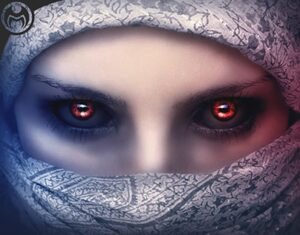
\includegraphics[scale=.5]{a20210703PassingThroughtheRealmsoftheJinn-img001.jpg}
\end{wrapfigure}

They frighten you with horrific appearances because they sense your hidden fears.

They tempt you because they see your secret fantasies.

They lead you astray because they know your unfulfilled desires.

Although they do not have real earthen bodies, they can nevertheless appear as physical bodies in various guises, such as animals, alluring women, or even terrifying images. In that regard they are like rainbows, which appear to be ``there" yet are not really there.

\paragraph{Facing the Truth}
The worse jinns are not those who frighten, deceive, trick, or tempt you. Rather, the worse Jinns are the ones who tell you the truth. We are each born with two angels assigned to us: one to guide us and the other to challenge us. Together they record our thoughts, words, deeds, and actions – both good and bad.

As we pointed out, to travel from the Earth to the Heavens, it is necessary to pass through the Realms of the jinns. Since there is no such thing as free passage, tolls must be paid along the way. The price is not in terms of money, but rather in terms of self-knowledge and purification of the soul.

At each tollhouse, the traveler is challenged. The two recording angels make the case for you, both pro and con. Since the jinn can read your soul, he will make the judgment. You will be allowed to pass on through or not.

Initiates understand this and undertake this journey while still alive and conscious. Since they begin the process of purification in this life, they are prepared for what they hear about themselves on the way. Everyone else puts if off until death when they no longer have a physical body help maintain balance. They are shocked about what they learn, especially those who pride themselves on being so spiritual and advanced in life.

\paragraph{The Final Reveal}
I can only speak from one side of this equation.

The jinn have often tempted you while disguised as women. That is because they can read your soul and know how your Anima image will respond. So if you think the women you meet are horrible, deceitful, etc. – as is not uncommon today in some circles—perhaps you need to look into your own heart.

Once past the Realm of the Jinns, you will need a new guide to lead you through the Spheres of the Planets. She is your Twin Soul, with whom your life is entangled and has always been. Some of you may know already who she is, but most probably not. So the truth telling Jinn will reveal your one true love to you. That can be the most frightening of all. That is the one opportunity that must be seized.



\flrightit{Posted on 2021-07-03 by Cologero }


%New thought
\chapter{Modern psychology: The Unconscious Mind}
\section{The German New Thought Movement}

\begin{quotationx}
This essay was originally published by \textbf{Julius Evola} in \emph{Bilychnis} in June, 1928. It is a review of the \emph{Neugeist} movement in Germany, which was derived from the \textbf{New Thought} movement in USA that had been developing previously. Now ``Neugeist" is the German translation of ``New Thought", but, following Evola, I have sometimes translated it as ``New Spirit" … Evola sometimes uses the German term, and others the Italian \emph{Spirito Nuovo}, a convention which I have followed. The essay will be presented in two parts. This first part is a general introduction. The second part will describe the actual exercises recommended by the New Thought Alliance.

These early articles from Evola that I have been posting demonstrate his spiritual quest, and are quite removed from the later preoccupations with politics, race, etc. It is clear, if readers will look back over the many reviews translated here, that Evola was willing to accept a form of Christianity that was ``practical", mystically inclined, and aligned more with Eastern teachings. Apparently, he was never able to find it, since he subsequently turned away from that quest. He even rejected what he, not incorrectly, called the ``vedantized Christianity" of Guido De Giorgio.

The other failed quest was Evola's search for ``special" powers, whether in the Tibetan Buddhists, yogis, or even the ``New Spirits". It is clear, given the number of references to them, that he was obsessed with the idea. Once again, all the magical exercises probably did not create those powers in the expected way. His correspondence with \textbf{Rene Guenon}, which was have made available, show this.

As for the German New Spirits, they seem to have disappeared without a trace; I am only familiar with Driesch, but only in a different context. I am sure that they were more intellectually sophisticated than their American counterparts. Since New Thought owed a certain intellectual debt to German philosophy, the Neugeist movement probably found a point of contact in it.

Of course, in a sense, they were on the right track. Thoughts do control our lives, that is why we deem it so important to understand one's own thought process. However, they seemed to have been inventing stuff on the fly without ties to a formal tradition. They retained the language of Christianity, but not its essence. As Guenon makes clear, the esoteric cannot be divorced from the exoteric, something that the New Spirits believed they could do. That is why the movement had to fail. On the other hand, a \textbf{Valentin Tomberg}, for example, managed to keep the esoteric and the exoteric together. That is the path to the future, the worthwhile way to ``change your life"; this path is immune to the petty criticisms of the dominant — and only — Western tradition that are heard in some circles. 

\end{quotationx}

In contemporary central Europe one of the spiritual currents that is gaining more ground, is that of the New Thought Alliance (\textit{Neugeistbund}). In essence, it is an offshoot of that reaction against religious dogmatism and scientific materialism, that that had already given rise to other more or less spiritual and mystical movements, like New Thought [in English in original], neo-Rosicrucianism, Christian Science, Anglo-Indian Theosophy and even spiritism. In regards to Neugeist there is however a sense of seriousness and enthusiasm not very common in most of these sects.

Not that it represents actually something original and united: on the contrary, there are clearly found in it ideas from Hindu yoga, medieval mysticism, and even classic German thinkers like Herder, Lessing, Goethe, Schiller, while on the practical side, the influence of the studies on autosuggestion brought in vogue by Coué and Baudouin is very clear. In spite of all this syncretism, in Neugeist there is a certain impulse that in a good measure unifies such elements close to an experienced need to bring man to recapture the sense of interiority and spiritual force.

The movement has its center in Pfullingen (Württemberg), where the editor J. Baum publishes the review Die Wiesse Fahne and a collection of small volumes among which in fact there are enough good ones (e.g., F. Eberspaecher, \textit{Der Giest sie Führer}, K. O. Schmidt, \textit{Selbst und Lebensbemesterung durch Gedankenfraft} and \textit{Wie knonzentrire ich mich?}, etc.). From Pfullingen, the movement extends especially toward Switzerland, Hungary, and Austria, where it has another organ: \textit{Das Neue Licht}, edited by F. V. Schöffel. There are among the adherents some rather noted names, such as Prof Verweyen and the vitalist H. Driesch.

Neugeist intends to be essentially a practical spiritualism, an active mysticism, with disdain for everything that is simple theory or belief. ``Neugeist", says Eberspacher, ``as vision of the world proceeds from this principle: that no knowledge has value if it is not applied practically; that the best ideas serve no purpose, if they are not transformed into action. Men must instill practically every day in life the teachings of a vision of the world."

The first opposition is naturally to materialism; in the second, to the ancient concept of faith and religion, which it wants precisely to replace with the New Spirit (\textit{Neugeist}). According to this ancient concept, says the author cited above, ``faith is nothing more than believing in undemonstrated propositions. Instead, for the New Spirit, faith is a force, by means of which the highest energies can be awakened." Dogma and confession are enemies and lethal for the spirit. Neugeist wants to be an \textit{``undogmatisches Tatchristentum"}, i.e., an active Christianity without dogmas.

At the center of its praxis, there is the concept of the sovereignty and power of thoughts. ``First of all, the most powerful of all forces lies in the force of though. The entire cosmos, all forms, and all phenomena, starting from the atom up to the solar system, are nothing if not materializations of the thought of God. Thoughts construct character, form bodies and faces, regulate health, determine our external relations, our destiny, happiness, or misfortune, the joy or sorrow of men. That which we form, shape, produce, is our creation from the inside—thoughts are the seeds, and the fruit is our fate, our good or our evil." (\textit{Schöffel in Das Neue Licht}).

That said, it is clear that attention is then brought to the techniques to make oneself master of thought in order to act, by means of it, in the direction of spirituality, elevation, and strength, on which it depends. Hence, the noted connection of Neugeist with the teaching of Yoga, with the modern practices of suggestion and autosuggestion, with the mystical disciplines of silence and meditation, purified however of their devotional or moral coloration and undertaken only from the point of view of their practical efficacy.

The inner journey given by Schmidt (\textit{Wie konz, ich mich?}) is divided into four major phases.

\begin{enumerate}
\item \textbf{Concentration}. This includes liberation, internal calm, ``Silence" and the concentration of thinking, feeling, and willing into a single point. 
\item \textbf{Meditation}, understood as the highest level of concentration in which man begins to direct thought onto a determined goal (concentrated meditation) and to make himself capable of keeping, this direction (pure meditation) fixed above everything, 
\item \textbf{Contemplation}, or inner mystical absorption, where the ear is turned to the ``inner voice" to which then one must try to identify oneself, proceeding then to the next level 
\item \textbf{Realization}, or self-completion, the level that precedes ``making oneself Christ" (Durchchristung), that is the highest stage of all the practices of the ``new Spirit". It is the same as ``cosmic consciousness" and ``being one with God" of all mysticisms. 
\end{enumerate}
We don't think it is without interest to reproduce some samples of the exercises used in the New Thought Alliance. The following are found in \textit{Die Giest sei Fuhrer}.

\begin{quotex}
Upon awakening in the morning, get dressed quickly. Turn to the East, extending the arms toward the Sun, draw seven complete breaths, breathing with the formula: ``Primordial creative force, fill me up." Feel the force as it floods you. Then cross your arms on your chest and say, or think, intensely: ``I am one with infinite life, its force fills me, today I will have full dominion over myself, I have its force. I am, I will, I can." Then say this formula in the same position: ``I send thoughts of love, peace, and harmony to the entire world, may all beings be happy and blessed." 

\end{quotex}
Another formula that is concerned more with the breath is found in Schmidt. Here the ancient Hindu doctrine of prana is understood, i.e., the mystical energy of life carried by the air.

\begin{quotex}
The air contains powerful forces that I introduce while breathing in. I draw these forces consciously. They flood my entire body and make me healthy, vital, free! They make me energetic and healthy! The forces restore me and animate me. I feel vital, energetic, healthy.

While exhaling, mentally and consciously chase away all the waste that has accumulated in your body, and at the same time, all the evil dispositions and impressions, negative and destructive thoughts. Think and feel: ``I breathe, I am free … free! I feel free — I am conscious, I breathe. Cosmic forces flood me and unite me to the Divine!" 

\end{quotex}
The repetitions, naturally, are made with the aim of autosuggestion. And now a formula for calm and inner silence. It follows exercises by which the complete relaxation of the body and every tension, almost to the point of no longer feeling it, are first stimulated. Again, from Schmidt:

\begin{quotex}
The external world has disappeared. I am alone, deeply in myself … I am silent, I am calm. I think and I feel that I am completely calm. Tranquility and calm are in me. Everything is calm rhythmic proportion, cosmic harmony, infinite peace. 

I am calm

Calm as though in a distant abandoned tomb.

Calm as though in the base to a clear transparent mountain lake.

Calm as though in a city underneath the heat of the summer sun, calm, tranquil, desolate, without noise, in anticipation of the freshness of the evening. 

\end{quotex}
Finally we translate a collective formula used by the Stuttgart group which was published in \textit{Die weisse Fahne}.

\begin{quotationx}
Om!

Rise up in me, you Conqueror of Death! Light of Christ! Infinite splendour of my soul!

You are! You dare! You burn up! In my soul. Light of Christ in me, I adore you!

In me was your Golgotha! In me is your Resurrection! Your eternal life lives in me! In me your paradise blooms! In me your liberation rejoices. In me your victory exults! In me your ancient flame shines. 

The Victor rises again!

You bring me back to the lost Father. You gave back the Father in me, who is also the Father of your original generation.

Your Father is also in me! Om! I am!

You, Lord, have risen again in me! New Spirit!

Ardent Spirit, resplendent with the original Light! Holy Spirit!

You who secures everything. You who hears everything. You breathe the world. You, the generator of the new Spirit. You the adsorbing Principal, to be bursting, the wise end, you, again the only Principle. You, the Everything and the Nothing, you, the One in Everything. 

You, the eternally active spiritual presence! Rising again!

Heaven jumps in me. The most sacred veil tears asunder in me. Your Light erupts from it. Your dawn Light of Eternity. 

In front of me, in me, every night!

Ancient Light, jubilant victory of the resurrection in me! Om! Victory! Victory! Victory! Om! Christ, you are the new spirit of Resurrection in me! Om! Peace! Peace! Peace is with us all! Om! 

\end{quotationx}
As you see, it is all rather well constructed in suggestive and intensely charged emotions in order to lead to a state of mystical exhilaration, not without certain character of virility.

What is interesting is to notice the scientific and, we would say, secular elements in the background, with which all the various means are syncretistically gathered in order to produce experiences, which are of value essentially from their practical efficacy. In other words, technique, in place of faith, and inner facts to acquire from pure individual experience, without dogmatic and profane ``interpretations", with an eye simply on their pragmatic ``truth" for those who demand a sense of exaltation of liberation of vital energy. Reaching to the foundation in this direction, one can expect that one day religion, as well as theology itself, will become an experimental science, certainly an upheaval, not lacking interest, that leads us back to a proper view of mystical and traditional esoterism.

These and similar movements are therefore observed with curiosity, as signs of the times. To the critic, for now it is more opportune to replace the watchful gaze that deepens the new themes that could begin to speak out in them.



\flrightit{Posted on 2013-12-04 by Aeneas }

\begin{center}* * *\end{center}

\begin{footnotesize}\begin{sffamily}



\texttt{scardanelli on 2013-12-04 at 21:45 said: }

``The first opposition is naturally to materialism; in the second, to the ancient concept of faith and religion, which it wants precisely to replace with the New Spirit (Neugeist)"

It seems that all such spiritual movements that are predicated on an opposition are doomed to failure. If the nature of this opposition is dualism then this dualism would make true transcendence impossible. This might also be applied to those traditionalists whose only rule for membership is being ``against" the modern world. 

Likewise for any attempt to strip Christianity of it's dogmas or confession. It seems to me that the truly esoteric should grow like a tree from the ground of the exoteric. The way of most new age movements is an attempt to usurp or get around the law rather than to develop and gain freedom from the law.


\hfill

\texttt{Anna Kaiser-Swadling on 2013-12-06 at 12:15 said: }

I've used something similar to the first ``auto suggestion" for many years. I find it empowering. Evola also has some techniques for falling asleep that I've applied for years after the ``I am alone, deeply in myself", i.e. visualising and moving toward a golden mountain peak, lying on your side and visualising you're looking from the back of your head, and another, lying on your back letting your eyes fall back then sense you're flipping back with them into the air above.


\hfill

\texttt{anon on 2013-12-07 at 04:37 said: }

This stuff showed up on my radar when I stumbled across Lisiewski, who hated New Age, but liked New Thought (NT). I woke up early today, and have been trying to find (online) the succinct Lisiewksi quote about NT that first impacted me, but to no avail. I guess these long ones will do. 

``You are the first of my readers to acknowledge that they have looked into that form of Mysticism referred to as `New Thought.' I am very happy you have indeed. You will find that—as I have written in the Magical Thought of the Week column weeks ago— Mysticism completes Magic: it is not the other way around, no matter how much this upsets people who are so entirely devoted to Magic. The entire matter of Spiritual `Unfoldment' as I term it—not Spiritual `growth' as the New Age insists—eventually leads to this end.

``Further, the amazing thing is that what the individual so desires; what he or she so sincerely wants or needs in their life, is all obtainable through this form of Mysticism, and ever so easily. Yet the paradox is that one cannot force one's self into accepting, working, and mastering New Thought simply because the results they require are so readily obtainable from it. Quite the contrary. One must `unfold' into it. And when that glorious days dawns, then all is made perfectly clear and works almost effortlessly for the individual so blessed with this `discovery.'

``People who are attracted to Magic must persist in it until the day comes when they `step over the line' that leads from Magic to Mysticism. It cannot be hurried. It cannot be rushed. But it will come. This is what Percy Bullock, one of the original members of the Golden Dawn Society meant, when he said at the turn of the 20th century, `In the end, we all become Mystics.' 

"Congratulations on your being attracted to it so early on. Perhaps—as sometimes does happen—it is the right—and only—Path for you to follow, even from the beginning."

– Joseph C. Lisiewski

—————————–

``My Reply: again, these individuals neither understand the difference between the `imaging' I teach, and the `visualization' which their New Age calls for. Nor do they understand the difference between one of their so-called `Invocations,' a `Prayer,' and an `Affirmation,' all of which I have thoroughly spelled out both in my books and on this website. And as the next reply will further show, New Thought has nothing whatsoever to do with `visualization' (in fact, those methods of New Thought that truly do work to produce full results have very little to do with Imaging either. That is, they employ Imaging only in so far as one forming the most `general thought template' of that which is desired.)"

– Joseph C. Lisiewski

—————————–

``Always use a nine foot diameter Circle of Art for every ritual and ceremonial act. `Nine' is the number of Yesod, of course, and corresponds to the subconscious (unconscious) mind, wherein all Magic truly occurs- we only `see' the results of that `occurrence' in the outer world (Malkuth.) That is, the subconscious mind should be thought of as the Causal Agent of the External Effect we wish to produce. There is a great deal of correlation between this concept and the central doctrine of New Thought. That is, with the extremely pragmatic philosophy and practice of the latter. But this is another matter for another time."

– Joseph C. Lisiewski

—————————–

``It may help if I give you an example. As I stated in Ceremonial Magic, I was born into a Roman Catholic family and raised in that Faith. And while I cannot abide the Catholic church in its present form, I yet consider myself a Christian, and more exactly, a Catholic! How can this be? Quite simply, I found the philosophical teachings of Pierre Teilhard de Chardin, a Jesuit Priest, theologian, philosopher, and paleontologist-and whose complex writing unify certain aspects of Science and Religion-to have a profound impact upon me. Together with the New Thought Philosophy, the two enabled me to form my own eclectic system of thought; one which is in perfect agreement with my own subconscious state of subjective synthesis, and which allows my magical efforts to succeed splendidly."

– Joseph C. Lisiewski

—————————–

``Apparently, they never heard of the work of Ralph Waldo Trine and his book, In Tune With the Infinite, which is regarded as the first independently published book on New Thought, and which is given credit for being one of the major works on the subject that sparked the New Thought Movement itself. And it was published in—1897! That is, his final manuscript, originally written in 1889, was published years before their famous Golden Dawn was being torn asunder by internal strife, and moving toward its ultimate 1900 collapse. Further, one has only to read Trine in the most cursory way to see if any `Golden Dawn' material—even theoretical—is in it. The philosophy of the Golden Dawn—and the Mysticism of Trine—are as different in theory and practice as are night and day.

``In the same vein, the people demanding I acknowledge the GD as having created the Mysticism of New Thought have no knowledge whatsoever of the existence and work of others in the field of mystical enquiry which has come to be termed `New Thought.' For instance: they apparently are completely oblivious to the late 19th century writings and teachings of Emilie Cady and Charles Fillmore, cofounder, who began the Unity Movement of circa 1890, the very time at which the first Golden Dawn Temple was getting underway in England. Formally called the Unity School of Christianity, the groundbreaking works of Cady and Fillmore—along with Trine's and a number of others less well known—constituted the initial creative impulse that launched the New Thought Movement.

``Further, unlike the bickering and backstabbing of the famous London GD Temple `elite' of the 1890's, enthusiastic collaboration between the schools of thought arising within the original New Thought Movement was the order of the day. Example: Emilie Cady—a staunch independent—published several of her most notable works in Unity Magazine, the official organ of the Unity School of Christianity in 1894-95 (these were then published as three paperbacks for the general public in 1896-1897.)"

– Joseph C. Lisiewski

—————————–

``But the Golden Dawn did has its effect, or so I speculate it did. That is, I cannot prove it empirically, but my research suggests more than a casual connection exists between the New Thought Movement and the original Golden Dawn as operated in England in the 1890's. And that is, that after the Golden Breakup in 1900, a plethora of new books arose on the subject of New Thought, the great majority of which suddenly began teaching `visualization' as part of their process. Not only that, but the visualization techniques they insisted upon are in every way exactly the same as can be found in any New Age book today—be it on Magick or on visualization techniques designed to bring about one's desires. For instance, the numerous works of Wattles (1902) Wilcox (1902) Towne (1904) Fritz (1906) Larson (1908) Sears (1919) Schubel (1922) and Van Resselaer Day (1928) are only a few of the many that initiated this unfortunate trend, while the latter works of Fersen (1929) Landone (1937) and Collier (1943) continued it. And of course, these later efforts were seized upon by the New Age and --‘expanded' into the non-functional miasma of so-called `New Thought' that generally exists today.

``In short, as the GD history states, most members of the original London Temple were `unknowns' who drifted away after the demise of the Temple. It may be that such people as Wattles—amidst dozens of others—were indeed members of the Order, or were acquainted with those who were. In either case, disillusioned due to the breakup of the GD, it is my opinion that they seized upon the New Thought Movement and added their `visualization' techniques to it, thus destroying the genuine techniques behind this form of Mysticism; techniques that indeed do allow New Thought—or `Higher Mysticism' as I term it— to work—fully, and without any Slingshot Effect. So much then for the people who lay claim that the GD `created' New Thought. As far as I am concerned, all that the (former) members of the original GD did to the New Thought Movement was contaminate it…"

– Joseph C. Lisiewski


\hfill

\texttt{anon on 2013-12-07 at 11:08 said: }

Warning: long and perhaps self-indulgent post follows.

———————————

Lisiewski's marriage of grimoires and New Thought reminds me, to some degree anyway, of those people who try to combine NLP with Crowley and/or with chaos magic. The whole Disinfo.com/RAW/Gen P-Orridge scene. Except that stuff is more modernist, I guess, whereas Lisiewski is relatively more traditional.

I read Jason Augustus Newcomb's ``21st Century Mage: Bring the Divine Down to Earth", years ago, and absolutely loved it. So much so that I joined his online forum for a while. And gushed words of appreciation at him. I couldn't get into his other book that was available at the time, ``New Hermitics". I had found a pdf copy of it, but couldn't force my way through it. It was NLP meets Leary meets Crowley meets RAW. Oh yeah, and hermetix too.

I remember when I first read an Anthony Robbins book, on the recommendation of someone I respected at the time, and thought to myself: ``This is magic." I never would have thought that. I saw Robbins as crass infomercial huckster. A bullshit artist. And I guess in many ways he is. But his neuro-associative conditioning (NAC) techniques are basically a form of crude and uncontrolled magic. Or something akin to it. As I played around with that stuff, those many years ago, I remembered the Sorcerer's Apprentice segment of the Disney cartoon Fantasia. Where Mickey Mouse casts a spell over some brooms, and then loses control over them. It was like that. NAC would allow you to effect change on the world around you. But this was done by first affecting changes inside you. And some of these changes were damaging, blinding you. Perhaps good for taking someone from tamas to rajas, but blinding them to many important aspects of sattva. Anyway…

Newcomb's Mage book is basically about the K\&C of the HGA, but in a sort of modernized and New Age-ified form. I neither know nor care if the practical suggestions that he offers in that book work. I already have my own practice. But the theoretical aspect of the book I found extremely and profoundly validating.

When you're navigating these meagerly-charted waters you need a compass. And the HGA provides that. Actually, I don't think of it as the HGA. As best as I can tell what people call the HGA and the K\&C of the HGA are really fragments of something much larger. Much more beautiful. The Abramelin operation, I believe, allows one to access only some of what is there. Like seeing an iceberg, and knowing that more is there under water.

Newcomb's book goes deeper than the HGA, but I'm not even sure if that is conscious on his part, or if his ``HGA" slipped some things in there, between the lines, in the connections between what he says, never fully spelled out. It's worth reading. 

Before I read Newcomb, I read one of the best books that I have ever read in my life. A book whose concepts still deeply nourish me, nine years later. When I found it, it was like the culmination and synthesis of a bunch of stuff that I was studying. I could not believe that such a thing existed. It was as though it had been created just for me. Of course, none of us are all that special, and any thought that has occurred to us, has also occurred to someone else, somewhere else. 

The book was like a synthesis and distillation of many aspects that I found most helpful and relevant in Jung, Tony Robbins, Crowley, Kabbalah, yoga, bhakti, chaos magic, psychology, New Age, religion and God knows what else. Plus I was physically chronically quite sick. And seriously worried about how the hell I the hell I was going to be able to support myself. I was working only part time. I was tired all the time. Low-grade fever almost all of the time. Heart-rate unnaturally high. All the time. Recovering from a very serious life-saving surgery. I did not seem to be getting better. I was afraid. 

The crass and cheesy title of the book is ``How to Get Lots of Money for Anything Fast". I have shared the pdf with significant people in my life, but none have had the experience with it that I have. Maybe it really is suited to a particular temperament? Or to people looking for a particular thing? Some are turned off by the title. Understandably. But the book really isn't about money. Or that is only the surface. It is about the K\&C of the HGA, although the author doesn't use those words. In practice, that is what it is.

The first time I did the exercises, it was profound. The strange chest pains I was having for some years, both before and after the surgery, were gone the next day. I kept expecting them to return. A week went by. Then weeks. Then months. Now years. The pains return only in periods of extreme stress. And that in very mild forms. Was it C.S. Lewis who said that pain was God's megaphone? I listen more carefully now, so I guess maybe He feels less of a need to shout as loud. 

The book is about navigating life, with the guidance of the HGA. Actually, something deeper, lusher and fuller than the HGA. Some will use that guidance to make money, but that is really like using a smartphone to hammer a nail.

But it can be used for that also. I remember an interview with Lichtman where he talks about something tho the effect that his idea was to provide a process whereby people could take care of their material needs simply and quickly, leaving time and energy for their spiritual pursuits.

My understanding is that there is a reality. Different people describe that reality, to varying degrees of accuracy. With varying degrees of clumsiness. Insofar as their gunas will allow them to perceive and describe it. Depending on what their goal is, reality can be sliced up in different ways, sub-divided into different categories. Some more misleading than others.

Lichtman calls his system Cybernetic Transposition (CT), being inspired in part, by Maxwell Maltz's Psycho-Cybernetics. But there is also a big dose of Lichtman's own spiritual beliefs intertwined in all of it. This troubled me somewhat, as his system goes deep into the unconscious, and I was worried about implanting some of Lichtman's own blind spots and perception-distortions into my own heart. 

So for a while I was really interested in what his path was. Finally, I was able to piece together who his spiritual teacher was. The dude's name escapes me at the moment. I could do a CT exercise to get my memory to cough up his name, but the important thing is that I found him both underwhelming, and mostly non-threatening. Maybe Lichtman has eclipsed his teacher?

Is Lichtman's CT Traditional? No, I wouldn't say that. And some of his blind spots I find loathsome. But I think CT can (largely) be used whoever one chooses. There is always a spiritual price to be paid with this kind of stuff, but I think CT fairly neutral, like logic. But then again, don't take my word for it. For all you know, I might simply be a self-deluded cultist.

Some of Lichtman's CT reminds me of a highly-fine-tuned version of chaos magic's sigilization process. Except done with words, paragraphs, vivid imaginary experiences. Instead of the commonly-used pictogram method. His ideas about getting the different parts of the brain working together, in concert, working towards the same end, cannot help but remind me of Kabballah's description of different parts of the soul. And also the Gita's vyavasay-atmika-buddhi. I will resist the temptation here to discuss the parallels between the source of buddhi and the functions of the HGA. This post is already long enough. 

CT has a bunch of controls built-in, to avoid having it blow up in your face, and for getting back on track. Since life is, in many ways, a moving target. You know now, things that you did not know then. And so on. 

This is not meant as an infomercial, or endorsement of Lichtman. I'm not getting paid for this. It's a genuine outpouring. Lisiewski has his New Thought, the Disinfonauts have their NLP Bandlerism. I prefer CT. 

Dig it.


\hfill

\texttt{IA on 2013-12-07 at 11:26 said: }

I've used daoist stretching, breathing and visualing techniques for over 18 years following recurring back pain from an injury. You face the sun every morning. It has worked very well for the back pain and may have some emotional effect as well.


\hfill

\texttt{pareidoliastic on 2014-08-11 at 11:48 said: }

anon on 2013-12-07 at 04:37, 

I have read all of Lisiewski's works and he helped open my eyes to Alchemy and Hermetics. After having a profound encounter with NLP in helping me literally evaporate an addiction I was trapped in. I am now very hungry for more and how NLP/NewThought could help me grow and evolve and get past all the other blocks from brainwashing and false beliefs I am clouded by.

I found this very page on the Internet because I to have a vague recollection of him talking about NLP and it's relationship to `magic/mysticism'

I have a great deal of trust in Lisiewski so his opinions and advice I give much more weight to than most.

From the quotes you gave he seems to indicate New Thought has been corrupted? Naturally because of the power these techniques have to modify the subconscious and influence ones subjective synthesis I am leery of just blindly following my natural instinct to read everything I can find on it. Other than his (apparent?) endorsement of Ralph Waldo Trine and his book, In Tune With the Infinite do you know of any of his recommendations on works for studying and working to find true liberation? I am also considering Hyatt's work in this area as I know he and Lisiewski were good friends.

Thank you, and anyone else who could perhaps aid me.


\hfill

\texttt{Cologero on 2014-08-12 at 07:51 said: }

pareidoliastic,

You are referring to some of the comments on Lisiewski, which were motivated by the translate essay from the German New Thought movement.

``True liberation" is not found just from studying, but from ``working" as you point out. It is not likely that much can be accomplished on one's own.

The danger is that before attempting to ``modify the subconscious", you should have a very clear idea of what you are doing. In other words, don't tinker with the mechanisms until you understand the inner workings of the soul quite well.

Originally, NT was based on certain philosophical systems, mostly forgotten because of the low quality of the NT movement. We have been discussing the intellectual foundations of magical idealism, which would serve as a better foundation. After all, what does it mean that representations create reality? We plan to revisit this theme in the next week or two.


\hfill

\texttt{pareidoliastic on 2014-08-12 at 15:19 said: }

Thank you for the reply Cologero. I guess the danger you mention is my trepidation about just `jumping in'. I understand the power of it now firsthand by using aspects of these techniques crafted by another to help root out destructive beliefs I had held subconsciously which made changing something the typical world thinks is nearly impossible. But it was actually quite easy. It has been said this person's book uses NLP so that rang a bell in my memory from when I studied Lisiewski's work and writings.

So naturally I am excited and very interested in how far that rabbit hole goes (in a positive sense) in how much greater I can truly be with the right constellation in my subconscious.

I have not really studied this site yet and what it contains in this regard. Can you kindly point me in the direction of the right place or post to dive into the stream on exploring this `magical foundation' theme you speak of?

And I look forward to your further posts on this theme you mentioned.

Many many thanks!


\end{sffamily}\end{footnotesize}

\section{Emile Coue}
\label{sec:Coue}
\begin{quotationx}
This is the promised translation of \textbf{Julius Evola}'s essay on \textbf{Emile Coué}. It originally appeared in \emph{Bilychnis}, in the Jan-Feb issue of 1925 under the title \textit{Emile Coué and ``Acting without Acting"}. Here Evola goes well beyond Coué himself and provides metaphysical, philosophical, and psychological explanations for the phenomena described by Coué.

Along with New Thought, which itself has been heavily influenced by Coué, couism, or something like it, has been a part of Hermetic teachings when properly understood. In reading this essay, perhaps some of you will be intrigued by this seeming paradox:

\begin{enumerate}
\item Coué demonstrated almost ``miraculous" results 
\item Similar results have been very difficult to reproduce 
\end{enumerate}

If point 2 were not true, then everyone would be demonstrating miraculous powers today. That I have not witnessed, not even in the New Thought circles that I was formerly part of. Yet point 1 has some truth, and Evola himself was convinced of it. Following the translation, we will offer an explanation of why points 1 and 2 are both true … unless someone else can explain it better. 

\end{quotationx}

The name of the Frenchman Emile Coué\footnote{\url{https://en.wikipedia.org/wiki/\%C3\%89mile_Cou\%C3\%A9}} has made quite a splash in recent times. There was a period in which, especially in France and in England, Couism had become the word of the day: a real interest and very lively discussion gathered little by little around the figure of this modern thaumaturge, his famous psychotherapeutic method of ``conscious autosuggestion", and the wake of almost miraculous healings left by his travels in the countries of central Europe and the New World. In these days, Coué has also come to Italy to hold a series of conferences that, if not of true enthusiasm—perhaps because of the rather skeptical nature of the greater Italian public—certainly has attracted much attention of the type which, among the observations of modern psychology of the supernormal, is always more inclined to believe that the power of man can in reality reach far beyond that which the small, humble, what everyday life shows us as possible in general. To tell the truth, the need that stands at the foundation of Coué's doctrine is rather important; it will therefore not be useless to attempt a reconstruction of it and, at the same time, to investigate up to what point the methods of Coué can be sufficient to it.

\subsection*{Section I}
The starting point, undoubtedly, is this. Hypnotic phenomena are real. Recent studies in this regard—it is enough to cite Liebeault, Bernheim, De Rochas, Richet—have truly been conducted according to the principles of the strictest positivism, and put the matter beyond dispute. Now it is factual that the hypnotized person realizes a number of things of which, in the normal or awake state, he is not absolutely capable: concerning perceptions, the emotional element, or various organic functions, he has a power that touches the miraculous. How is that possible? Here we have the first position of couism, expressed in the principle—moreover already announced by Liebeault and Myers—that \textit{every heterosuggestion (i.e, a suggestion made by another) is realized only through an autosuggestion}. That is, the theory that the power of the hypnotizer works directly on the hypnotized person is excluded. The hypnotizer only transmits a command, he only suggests the idea of the thing to be accomplished: but in order for the suggestion to be effective, it is necessary that the subject assume it, transform it into an autosuggestion and thereby realize it with his own strength. Receptivity is in fact an essential condition for the success of the suggestion. It would follow from that that the operative power in the phenomenology of hypnosis must be pushed back not to another, but to the I itself: that, at least, in its material aspect of a force ``that does", aside from the principle of the impulse that causes it.

It must be placed back on the I, so far, so good. But which I? Clearly not the I of the conscious personality: the hypnotic sleep effectively entirely abolishes such an I. It therefore necessarily pertains to another, deep power of subjectivity beyond that which consciously thinks and wills, a much vaster and stronger power that Coué designated sometimes as the \textit{imagination}, and at other times—following Jung—as the \textit{subconscious}. Now in the phenomenon of heterosuggestion these two I's fall into two distinct beings: in the hypnotized person, the unconscious principle and realizer; in the hypnotizer, the conscious and directing principle. The problem that couism poses is this: to substitute the I of wakefulness for the hypnotizer and to reunite the two principles in the same subject. Hence, the concept of a suggestion to be made by oneself to oneself, according to directives that the I of awakening should formulate and the subconscious carry out: hence, the theme of \textit{conscious autosuggestion}.

Before going further, let us lay down a more precise understanding of what the subconscious is. Here Coué—keeping in mind what the subconscious shows us it is capable of in hypnotic phenomena—refers to an entity that presides over \textit{all} organic functions, from the most humble of the vegetative life to those that govern the mental processes themselves, and, therefore, it corresponds to entelechy as described by Aristotle and Driesch, the ``\textit{logos}" of Sthal, the ``physical personality" of Ribot. But this determination is still exterior: it does not tell us what such a principle is in and for the I. And that is must be something for the I, which it in one way or another must emerge, must be put at the head of the luminous zone of consciousness, which is clearly presupposed by the problem of conscious autosuggestion: since if the two I's were such that they mutually excluded each other, or that when the subconscious emerges the consciousness is submerged and vice versa, it is clear that the action \textit{ab intra} that couism proposes would not be possible.

Duality must therefore be in a certain way present in the very sphere of the life of awakening. To that we refer to Coué's other term, the \textit{imagination}. He notes that in the same conscious life, two entirely distinct powers are in play: one relates to the plane of intellection, the clear consciousness and reflective will; the other to the murky reign of the instinct, emotion, passion, and deep and irrational convictions whose dominant principle is that of faith and imagination. The one is, to use Platonic terminology, the \textit{logos}, the other, \textit{eros}. Coué distinguishes rather cleanly between these two powers: they have individuality and absolutely heterogeneous modes of acting. Now while the logos falls outside that deep principle that rules the whole of organic functions, the eros communicates with it so that, in a certain way, it is identified with it. The corollary follows immediately from that—the key point for couism—that the problem of the control of one's own personality—and that not only with regard to the element of character, but also with regard to the physical being and, therefore in particular, the problem of eliminating psychic disturbances and maladies (psychotherapy)—it is mutual with that of the determination of the eros from part of the \textit{logos}, for the ``imagination" from part of the conscious I. This is the task of conscious autosuggestion: to succeed in making directives originating from the I from the imagination accepted, so that they moreover become directives for the organic subconscious which, blind and inert, cannot fail to obey them as it happens in hypnotic phenomena.


\hfill

\begin{quotationx}
This is part 2 of \textbf{Julius Evola}`s review of the movement initiated by \textbf{Emile Coué}. It would be curious that Coué discovered all these techniques himself, since they are part of Hermetic and magic training. Here are some of the salient points to notice:

\begin{itemize}
\item A monoideism is a state of focusing the mind on a single idea as in hypnosis. Negatively, it is related to the ``idee fixe" described by \textbf{Valentin Tomberg}, or more colorfully, and not completely inaccurately, as ``possession by a gnome". Positively, it is an aspect of deliberate concentration exercises. 
\item Man, as he is, i.e., the man untrained in mental or spiritual development, is not as conscious as he believes himself to be. Rather, he is a ``puppet" under the domination of myriads of suggestions, most of which do not emanate from himself. 
\item The so-called conscious mind, i.e., the discursive intellect is a mass of contradictory ideas which very often impede our lives. 
\item There is a deeper ``I" or self, beyond that seemingly awake I, that is the true and real source of our lives. 
\item That deeper self responds to suggestions arising in the conscious mind or those entering the conscious mind from outside sources. 
\item To ``reach" that deeper self, it is necessary to somehow suppress the incessant chatter of the conscious I. That is the real goal of meditation, concentration, and other so-called magical techniques. Even ``sex magick" has nothing to do with sex, beyond using it as a means to bypass the conscious mind. 
\item Notice, for example, how Coué's ideas track the notion of ``concentration without effort" as described by Valentin Tomberg. 
\item It is clear that these techniques sound simple, but are quite difficult in practice. That would account for the seeming lack of success in most cases. The state of ``conviction", faith, or the ability to ``will one thing" is elusive to those who think too much. 
\item Based on the examples that Evola provides, perhaps the purpose of these tests for \textit{Qualifications for initiation}\footnote{\url{https://www.gornahoor.net/?p=1161}} may be clearer. 
\end{itemize}
\end{quotationx}

Since autosuggestion is possible in principle, Coué sees it confirmed by a thousand facts of daily life. Three fourths of our actions —as he claimed to one of his disciples— are, more or less directly, supported by autosuggestion: only that we habitually suggest to ourselves without either knowing or willing it and, in most cases, as though it were all our doing. Here Coué emphasized the opposition of \textit{logos} to \textit{eros}, he often loves to highlight how our conscious will and reason can do nothing against an autosuggestion, since what makes us act is always the imagination. He says,

\begin{quotex}
When the will is in battle with the imagination, it is the will that, without exception, loses the game. 
\end{quotex}

Not only that, but the efforts made by the will in similar cases succeed simply in reinforcing the power against which it faces. This is the \textit{law of reversed effort}. Examples:

\begin{enumerate}
\item The novice bicyclist sees a stone in the middle of the road, he \textit{imagines} that he is going to run over it, he \textit{struggles} to avoid it; the harder he tries, the more likely he goes right over the rock. 
\item A person notices he cannot fall sleep; he wants to sleep: the more he wants it, the more he does not succeed in falling sleep. 
\item A sufficiently large plank is placed across an abyss; if the same plank were place on the ground, a person would walk across it with the greatest nonchalance. But being placed over the abyss, he \textit{imagines} he could fall; he does not then dare to traverse it: if, in spite of everything, by forcing an effort, he attempts it, in the great number of cases he is going to fall off. And so on. 
\end{enumerate}
These and numerous other examples show that the will can do nothing against a present suggestion. The secret of success is instead to oppose a suggestion not with an effort, but rather with another suggestion of the opposite meaning: it is necessary, i.e., to translate the will into a corresponding ``imagination". Without that, the effort succeeds only in precipitating the occurrence in the direction opposite to the one desired. Therefore Coué says:

\begin{quotex}
We who are so proud of our will, we who believe we freely do what we do, we are in reality only poor puppets of which our imagination holds all the strings. We cease to be these puppets only when we have learned to guide the imagination.
\end{quotex} 

Here we can make a rather important observation about the mode of action of the two principles. In apparent contrast with what at first view would let us think of the classifications of logos and eros, we see that the mode of the first is action properly called, or effort, tension; in contrast, the mode of the second is purely mental, it is an ``imagining", a sudden and inner, effortless, self-representation. This pure ``imagining" realizes, and realizes it to the very depths of the one's being: instead action or will, purely called, is condemned to the periphery, and can do nothing in respect to the deepest stratum of the physical and emotive personality, and when it intervenes, it succeeds only in leading to battles and disagreements with almost always detrimental consequences.

The problem therefore is centered in the question of provoking consciously and intentionally that autosuggestive process which, in the background, plays such an essential part in daily life: or, in other words, of discovering the method by which one can act on the ``imagination" starting from the I of awakening. Coué's principle in this:

\begin{quotex}
every idea that engages the spirit exclusively becomes ``true" for the imagination; the concentration of the mind on an idea transforms this into a belief. 
\end{quotex}

In technical terms: it is about creating in oneself a ``monoideism". Faith and monideism, ultimately, would be equivalent to each other. That said, the technique of couism is the following:

\begin{quotex}
The principles of the will and the imagination exclude each other; in the hypnotized person the power of the subconscious is so great because a free field is left to it, while everything that is related to the will and consciousness is put aside. The ideal would therefore be the ability to enter a hypnotic state: but since the hypnotic state suppresses the conscious I by hypothesis, it is necessary to find a compromise, viz., of the intermediate stages in which the surfacing of the subconscious has the maximum, compatibly with the minimum permanence of the conscious principle. 
\end{quotex}

Such are the so-called ``hypnoid states", among which Coué emphasizes that of \textit{détente} or relaxation. It is a matter of realizing a complete relaxation of the conscious faculties, of excluding every mental and muscular effort or tension, just as happens immediately before falling asleep and in so-called \textit{reveries}. When the mood of \textit{relaxation} ends up sufficiently incited, the conscious principle that up to that point was put aside—withdrawn almost to the extreme corner of oneself—it can intervene and make the idea slip into the mind, or better put, the \textit{image} of what one desires to realize. The mind must fixate on this image to the exclusion of all the rest, moreover without entering into the field of efforts, which would destroy the state of \textit{relaxation} and, along with it, the state of receptivity and of suggestibility of the ``imagination". How then can one realize such concentration? Coué's answer is:

\begin{quotex}
By means of the very rapid repetition of a formulation which includes the idea in question; with the repetition, the mind is automatically and spontaneously brought to the idea, and its speed makes it such that other images are not inserted in the intervals. In particular: any counter-suggestions are not formed which would neutralize it and thereby render it ineffective. Through repetition, monoideism is formed: absorbing the whole spirit, the image strengthens itself slowly in the imagination until it becomes a dim and deep conviction; it is then employed by the power of the subconscious from which it certainly is turned into action. 
\end{quotex}

If, e.g., in a hemorrhage, one succeeds in concentrating on the formula ``the hemorrhage has stopped" —like a mood freed from conscious faculties—, to the point of rendering itself fully active, the related image lives in the mind—in a word: to the point of believing it, then this idea becomes a truth and a command for the subconscious that, as director of every organic function, makes the arterioles and venules contract naturally, just as would happen artificially with a tourniquet: and the hemorrhage is stopped.

This, in a few words, is Coué's theory. In experiments, it seems to have been demonstrated as capable almost of a miracle. Limiting ourselves to the physio-pathological order, to which it particularly is oriented, not only functions but also organic paralyses, advanced stage consumption, generalized eczema, tubercular lesions, tumors, etc. have been cured, sometimes in very few sessions, by means of the autosuggestion developed from the illness itself under the guidance of Coué or his disciples.


\hfill

\begin{quotationx}
In Section II, \textbf{Julius Evola} offers a critique of \textbf{Emile Coué}`s explanation for the successes of his method, and then provides his own explanation.

Making the connection between the ``deep conviction of the subconscious" and ``faith", Evola then relates it to the ``vexed question" of ``grace". In other words, why do some have faith and others do not? Or, in more practical terms, why are some healed by couism while most are not? However, Evola here is interested only in a psychological explanation, not a metaphysical one. So ``grace" means only that its origin seems to come from outside rather than from one's own powers. This is a different question from the metaphysical meaning of grace.

First of all, while faith is the belief in something unseen, it is more than that since it reaches deeper that our everyday I that we consider to be conscious. This I, however, is engaged embroiled in dualisms: subject-object, true-false, right-wrong. The deeper I, on the other hand, is non-dual: it simply is and it wills one thing. There is a certain seemingly ``heroic" attitude that sees doubt as concomitant with faith. But that is to remain perpetually at the level of that ``I of awakening" while never penetrating to depths.

Rather, the proper development of faith is gnosis, i.e., the direct realization that has been mentioned several times in Evola's essay. In this regard, Valentin Tomberg is a more reliable guide as we have shown in \textit{The Elements of Sacred Magic}\footnote{\url{https://www.meditationsonthetarot.com/the-elements-of-sacred-magic}}.

To his credit, Evola does not deny the numerous preternatural and miraculous accounts of the saints, and, growing up in Italy, he would have heard of many. Therefore, he rejects a glib positivism that rejects miracles out of hand. In contrast, he develops a ``metaphysical positivism" that would account for the reality described in those stories. Nevertheless, in the final analysis even metaphysical positivism leaves out something essential.

He rightly rejects the claim that the method of couism is sufficient in itself, apart from the person of the patient. Otherwise, if the method worked indifferently, there would be couism centers in every city instead of hospitals. At some point, it is up to the patient to develop faith or the image of his healing. Every suggestion, to be effective, eventually becomes an auto-suggestion. Not only the belief in couism, but also the belief in any ceremonial, ritualistic, sacramental, or symbolic forms have no power in themselves other than to motivate faith in those who need it.

Some, however, do not require any such aids. This would mean, fundamentally, that a man can do without a Tradition. Such a man, however, would not know what to have faith in, and hence would not find gnosis. Typically, he would actually be a secularist. The symbols cannot be discarded so readily. Yet, any psychological explanation can never be complete as long as something supernatural or transcendent remains unaccounted for (which it must, in psychology).

Nevertheless, Evola's emphasis that a personal realization is somehow always involved and that repetition for its own sake is useless is sound. Yet, there is one miracle that Evola's purely psychological explanation does not capture. That is Peter's raising Tabitha from the dead and the dead, presumably, are immune to a hetero- or auto- suggestion.

\end{quotationx}

\subsection*{Section II}
The great problem that comes into play in couism is that of the construction of faith. In fact, it becomes clear to everyone that that deep conviction of the subconscious that Coué speaks of is nothing other than faith. Fundamentally, it comes back to the vexed theological question of grace. The principle that faith, once reached, is an irresistible power, which immediately realizes what it believes is true, has been known from the most remote times and, at least in a certain measure, has since been scientifically sanctioned by modern psychology. And the significance of faith is not only subjective, it is also objective. The accounts of the miraculous phenomena that envelopes the figures of saints and creators of religion — so lightly discarded by so-called positivism — in reality take inspiration from faith. Of the similar phenomena of yoga and magic, the principle, in the final analysis, is faith or, if one prefers, autosuggestion. Explanation:

\begin{itemize}
\item At the first level, I can have the simple, empty concept of a thing. 
\item Beyond that, I can bring it to life in the imagination. 
\item In the third place I can perceive it exteriorly as a subjective hallucination. 
\item In the fourth place, I can act on other consciousnesses in a way that they also perceive it (collective suggestion). 
\item The \textit{same} power, continued in an ever more intense affirmation that invests the level of physical being, becomes objective and, as such, is a magical act. 
\end{itemize}
As the mage can be defined as the one who knows how, so to speak, \textit{to influence the same nature}, to communicate his faith to it, with which one is preliminarily put in relationship by means of an act of love or sympathy.

However beyond that, the great question is to know \textit{if}, and in this case, \textit{how}, faith can be constructed positively and consciously by the I, and, to tell the truth, beyond any suggestion whatsoever. In the great number of cases, it is to be noted that the I does not possess faith as much as it is instead possessed by it. I.e., in them, faith is realized to the extent it does not flow from an absolute sufficiency, from a pure self-assertion of the individual, but from the suggestion derived from some idea, close to which the I originally — in the moment in which it was triggered — is passive and unconscious. So that if it is true that no suggestion (hetero-suggestion) succeeds if it does not make itself an autosuggestion, it is also true that, almost uniformly, no autosuggestion (with particular regard to those that can extend the power of the I beyond normal) is actuated if it does not have a preliminary suggestion as a basis for motivation. That is, the I does not succeed in being present, to assert itself at the moment of the initiative. So the person of faith at Lourdes, in as much as it heals, to that extent he believes that it is not he, but divinity, who works the healing; to the extent the hypnotized person carries out miracles, to that extent the initiative, the suggestion, comes to him not from himself, by from the hypnotizer. And that, to tell the truth, can extend to a great number of Coué's patients, who heal to the extent that they believe either in Coué, or in the efficacy of the ``method", or, at least, in the existence of the ``subconscious", that he, and not themselves in naked individual affirmation, will know how to heal them.

Actually, for example, one would like to see if the healing of so many persons —\textit{after Coué's invitation}— as soon as they affirm that they are cured, would have likewise occurred if it were any of the readers who made that invitation to them. On the other hand, we must note that the various miracles of the saints, at least in Western mysticism, were experienced in the spirit of the intervention of a higher and transcendent power. The same magic is related to the whole of ceremonial, ritual, symbolic, etc., manifestations which are only the necessary substitute for those who do not know how to create the powers of the imagination by means of a positive central initiative, but attain them only indirectly by virtue of the suggestion emanating from a complex of extrinsic elements. Nothing other than this absence of oneself from the principle of a positive initiative, this incapacity to create faith \textit{kath'auto} [in himself], gives the meaning to what is indicated as ``grace" in Western theology. However, even if there is grace, conscious autosuggestion is a useless name: for the starting point, it has an unconscious autosuggestion (a hetero-suggestion)—a mystery and a passivity; and then the I appears the instrument of faith, not its creator and the possessor.

Such therefore is the true light under which the requirement emerging from couism must be examined. Now the idea that for the construction of faith an automatic repetition of formula in a state of relaxation is sufficient, is rather ingenuous. First of all, we must note — as was done above — that a great number of persons who succeed with such a method are already hetero-suggested, directly or indirectly, by Coué or by those who tell them about him and his doctrines. In the second place is the fact that the \textit{imagination} or faith is \textit{invariably presumed in itself}; i.e., one does not achieve it starting from something different from it, but rather starting from an initiative that resides in it and not in the peripheral faculties of normal consciousness. So that it is said: ``The blind man does not have any possibility of making himself a guide." If the repetition is simply mechanical, if it is not already accompanied by a certain level of interior evidence, it results in nothing, and regarding that, anyone can perform the experiment whenever he wants.

In the East, where these things were studied at their foundation, they likewise recognize the importance of \textit{japa} (repetition) through the ``realization" of the so-called mantra (magical formula); however, it is explicitly said that one can do \textit{japa} even a million times, but unless the mantra is ``understood", ``awakened" (\textit{sphota}), the \textit{japa} remains a mere flapping of the lips. This ``self-awakening" of the mantra is an illuminative moment; of pure inner evidence (so it is said in the texts that ``awakening" the mantra means to realize it in one's essence ``made of light", \textit{Jyotirmaya}), which can be propitiated and intensified from repetition, but not generated, for that demands a true spiritual spontaneity, an effective passing of consciousness from one ``dimension" to another.

It is a question of the same qualitative heterogeneity that intercedes between the concentration of the fire of a lens over a substance and its sudden burning up—naturally considering the phenomenon not from the physical point of view, but from that of the psychological effect in a spectator. Therefore, it is not necessary to have any illusions of the efficacy of the ``method": one can be certain that wherever it succeeds without a true initiative or inner conversion coming into play to animate it — of which very few are capable — it succeeds not through its own power, but rather through some hetero-suggestion that unconsciously is insinuated into the process. And then, from the practical point of view, the result will be equally good: its spiritual value, in reference to the previously mentioned problem, is therefore nullified.


\hfill

\begin{quotationx}
This is the final installment of \textbf{Julius Evola}`s essay on \textbf{Emile Coué}. Section I was an overview of couism, Section II dealt with it from the psychological point of view, and Section III analyzes it from a metaphysical or spiritual point of view.

The spiritual level overcomes all dualities, so force cannot be understood as working against an ``outside" object. Rather, the unmoved mover ``acts without acting" in the Taoist and Aristotelean sense. Therefore, in conceiving or imagining something, it brings this about ``without effort". Thus, Evola claims that couism needs to be raised up from the unconscious. The ``imagination" is a higher faculty (it is one of the ``wits" or internal senses. See, e.g., \textit{The Phenomenology of the Medieval Mind}\footnote{\url{https://www.gornahoor.net/?p=3559}}).

In this state, Evola claims, one will have power not just over the body and its vegetal functions, but even over physical nature. Unfortunately, couism itself is just a tool and not a road to get to that state. For that, ``faith" is necessary. But faith in what? Does the ``I" simply believe whatever it wants, or is there really a transcendent revelation that is necessary? Here Evola seems to fall short. As long as the quicksand of the subconscious is full of ``obscure and murky" ideas, the I cannot lift itself by its own bootstraps from that trap. 

\end{quotationx}

\subsection*{Section III}
In order to specify the meaning of that change of interior level, we can add the following observations. A rather profound truth stands behind the opposition of the will and imagination. We are accustomed to consider force as a near synonym to coercion, to reduce the will to mean \textit{muscular}, but that however presumes an antithesis, a resistance (whether physical or moral), which the I faces and struggles against. All of so-called Western ``activism" is based essentially on the concept of tension and effort. Now such a concept of action is fundamentally inferior. Referring precisely to this idea, Lao Tzu was compelled to indicate the mode of spiritual power as \textit{wei-wu-wei}, or acting without acting. It is important to understand this point well.

It finds its best illustration in the Aristotelian concept of \textit{akineton kinoun}, i.e., of the unmoved mover. The one, who is really the cause, does not move: he remains firm at the point of pure creative initiative. Movement takes place only in the effect, in what proceeds from him and of which he remains the master and calm director. In this sense he, properly speaking, does not act: he conceives—he only produces the movement, he causes action without being dragged into the movement and passion, without engaging himself, but \textit{effecting} it and dominating it. Such is the meaning of \textit{wei-wu-wei}.

The same idea is found in the Shakti Tantra. The moment of the permanent (Shiva) is in the positive or masculine power, and the negative, or feminine is that of the dynamic and active power (Shakti). This is in open contrast with the western views which, having lost at this point any trace of the higher mode of the spirit, consider action relating to the simple demiurgic force, passion, manias, mere actuality or spontaneity as positive and masculine, i.e., having its own principle outside itself (and such is the truth of the ``evolutionistic" doctrines such as those of Bergson and Gentile). This is, actually, to be called passive and feminine. Hence, even the deep sense of the opposition, in Christian Gnosticism, of the ``pneumatic God" to Yaldabaoth, the demiurge God and creator.

The spiritual, by hypothesis, is superior to every antithesis or polarity; the material is instead formed in it and for this reason, its principle is struggle. The same concept of force—just as Guyau correctly noted—arises outside of the relationship to a resistance, so that it, in an absolute way, does not indicate potency, but impotency. Instead, the spiritual never needs to ``struggle", it unfolds in a calm way without fighting. Hence, the profound meaning of the paradoxical aphorism of Lao Tzu, that ``truly victorious army is the one that has never fought."

It is a matter of an inner and subtle action that is irresistible since it is part of the level of a principle, that has nothing against itself, that is entirely and hierarchically superior to every antithesis and polarity of the material or moral plane. This ``creative indifference"—as Friedlander-Mynona calls it—that is pure, subtle conceiving, is referred to again, in the Kabbalistic tradition, and the eleventh Arcanum of Force in the Tarot, in which the symbol of a woman holds tight the jaws of a furious lion \textit{without any effort}, exhibits, precisely the manner of spiritual causality, the mistress of every violent force and every physical determinism. On the other hand, the Lodge, it is in the curious words: ``he walks with a stick; therefore rifles discharge with a wave of his hand."

Now, it is precisely such acting without acting that it is necessary to refer to when Coué speaks of the ``imagination": the world of this imagination, just as we expressly mentioned, is indeed not an acting in the proper sense, but instead a self-representation, a pure, interior apperception — something that becomes, insensibly and subtly, almost from nothing. The will is, to tell the truth, a principle connected to the physical being and the environment, a product of biological contingencies: it therefore necessarily submits to the limits and the conditions of the life of relation and the material plane. In the ``imagination", the reflection of ``acting without acting" is instead expressed, or acting without effort for higher spiritual spontaneity. In it, the I can therefore have a true magical organ, an organ by which it can assert itself over whatever eludes the willpower in the strict sense: over its emotivity and over its physiological being, and not only, but even— this affirmation does not seem too audacious—over physical nature.

The day will come in which one will realize that everything that man realizes by means of positive science over nature is only an illusion of power: in fact, it does not truly dominate in the various mechanisms devised by technology, but makes itself the slave and always more dependent on the various natural laws that it presupposes, recognizes, and exploits. And that is because the scientific attitude is essentially extroverted and separative and because its level is that of the I opposed to the non-I and not that of the principle that understands this duality and is interiorly superior to it. The secret of our impotency is precisely this: that we are preoccupied by things, that our action is almost magnetized by them, that it never truly draws its determination from its own interiority. We put ourselves on the same plane of phenomena or the outer world, although we are subject to its laws. Should one instead place himself for an inner conversion at the level of that which rules phenomena, what external thing could no longer be resisted? Now in ``faith", ``imagination", etc., there is precisely a suggestion of such a level. If we would know that we do not see or act relying only on a pure affirmation or inner certainty, then we would unlock the realm of the only real power. This is active faith: the popular saying that faith is blind is spot on. But such blindness is not a privation, it is instead a perfection; it symbolizes the pure freedom where the ``seeing" here would signify it was tied, it was subject to the law and the principle of the ``other".

Coué's merit is therefore to have brought to light the inferior, negative character of the will properly (or improperly) called, in general, that of violent and antithetical action against the subtle mode of a realization without effort that, to tell the truth, stops being ``sensible". His defect is not having understood ``imagination" as a higher level of the spirit, but of having substantialized it superstitiously in a type of distinct entity opposed to the conscious I, to be used via small expedients. His method acutally does not center on the I in the role of the ``imagination", but seeks instead to excite it from the outside through the technique of relaxation and repetition. Thus, in order to empower the conscious individuality, to elevate its pure energy to the luminous peak of a pure act, couism estranges the I from itself, doubles it in a type of hysterical dissociation. Then the imagination adopts the obscure murky power of the subconscious, studied by psychoanalysis that, in such cases, has this advantage over cousim: it seeks to penetrate and resolve it in clear consciousness, where cousim does not care about that, but only to make it work. And such a scission, admitted in principle, brings a serious consequence. If the subconscious then comes about as a distinct entity, man will also be able to dominate with it this or that element that previously eluded him, he will also be able to make his warts and his asthma disappear, but never will he be able to guarantee an autonomy to what he wants and that he can only be the effect of obscure subconscious processes, which he does not know, nor can he know anything about them.

The same reasons in the name of which he could use or subject the subconscious—given also that he succeeds in it — would be able in their turn to be just the symbols of subconscious impulses: every freedom could be only the peripheral appearance of the instrument of an irrational and impenetrable force.

This essay on couism and its problems that arise from it suffices for now. Everyone sees that it is a matter of passionate questions, which would merit being considered and amplified rather more than what has so far been done.

\hfill

\flrightit{Posted on 2013-12-16 by Aeneas}

\begin{center}* * *\end{center}

\begin{footnotesize}\begin{sffamily}

\texttt{scardanelli on 2013-12-19 at 10:41 said: }

Thank you for this translation Cologero. It has been extremely useful to me in clarifying Tomberg's third letter and the concept of sacred magic.

Here's wishing you and your family a Merry Christmas. I offer my prayers for health and wisdom for you and all of the readers of Gornahoor.

``Thou, chaste Moon, full of joy,

Favour, since thy Apollo now reigns,

The Child who was born this day.

He alone will cast iron out of the world

And populate both Poles with

A most precious lineage of gold"


\end{sffamily}\end{footnotesize}

\section{The Healing Power of the Mind}

Although \textbf{Emile Coué}, who originated the affirmation, “Every day, in every way, I am getting better and better”, may not be so well known today, his influence is nevertheless very great indeed. Anyone on facebook cannot help but notice the constant flow of “positive affirmations” in his feed, which is undoubtedly part of Coué's legacy. While I agree it is fine to think positively when appropriate, it often rises to the level of superstition. I knew a woman who refused to dance the tango with me because she felt the music was too sad.

It may even become delusional when the hard facts of life confront us. Prince Siddhartha's life was totally altered when he came to terms with illness, ageing, and death; positive thinking alone cannot prevent them. In the teaching of the dominant religion closer to home, the loss of the Primordial State brought death, toil, and pain to the human race. The solution to death has to come from the outside, not from nice thoughts.

Evola, however, was quite interested in Coué and devoted a longish essay about his teachings\footnote{See Section~\ref{sec:Coue} in this book.}. Evola related Couéism to the “acting without effort” of Taoism, using language not unlike \textbf{Valentin Tomberg}'s description of the Juggler or Bateleur\footnote{\url{https://www.meditationsonthetarot.com/personal-effort-and-spiritual-reality}}. But before offering up the translation of that effort, I would like to provide a little background for comparison and contrast to Evola's views. On the one hand, we will use some concepts from German philosophy to make a plausible case and also Fr. \textbf{Alois Wiesinger}'s comments from his book \emph{Occult Phenomena}\footnote{\url{https://www.gornahoor.net/library/occultPhenomena.pdf}}.

\paragraph{The Soul Principles of Healing}
Fr. Wiesinger devotes several pages to Couéism. First of all, he notes the well documented possibility of the healing disease through interior powers. This is not implausible when we recall that the body is the form of the soul, so that changes in the soul life can and will affect the body. As a trivial example, we can note how erotic thoughts effectuate bodily changes. Fr. Wiesinger notes that

\begin{quotex}
there are in the subconscious those purely spiritual powers of the soul which are remains of preternatural gifts. Sometimes these can achieve wonderful results. 

\end{quotex}
There two principles that account for Coué's success:

\begin{itemize}
\item Every thought strives towards its own realization 
\item The law of effort produces an opposite effect. 
\end{itemize}
In the first law, the more a thought is entertained, the more the nervous system will seek to realize it. That is, the sense-stimulus nerve system will create a pathway for the motor nerve system. There are some drawbacks, the most obvious of which is that the vegetative soul is not very responsive to conscious control. (E.g., you don't digest your food by thinking through the process of digestion.) The other more subtle one is that every thought engenders some doubt, which may negate the original positive thought. Hence, Coué turned to the subconscious for the second principle. Fr. Wiesinger explains:

\begin{quotex}
When the will commands an act, then the reason judges whether such an act is possible, reasonable, useful, etc., and so by its doubts and reflections prevents the first law from being effective. 

\end{quotex}
Hence, the positive suggestions need to take place in an altered state, i.e., a “half-sleep”, or “alpha state”, and so on. That is why so much operative magic relies on techniques to quiet the conscious mind in order to reach down into deeper states. These states are more receptive to autosuggestion and don't give rise to doubts. The modern Westerner is too dependent on reflection and the conclusions of science, so he finds it difficult to reach such states. Hence there results a self-fulfilling prophecy. This is unlike Jesus' teaching recorded in Mark 11:23:

\begin{quotex}
Amen I say to you, that whosoever shall say to this mountain, Be thou removed and be cast into the sea, and shall not stagger in his heart, but believe, that whatsoever he saith shall be done; it shall be done unto him. 

\end{quotex}
Although Fr. Wiesinger devotes several pages of examples, including those from Christian Science (a close relative of New Thought), we can skip past them for our purposes. The main points of interest are these:

\begin{itemize}
\item To be effective the discursive mind must be repressed. Evola refers to this as the First Trial\footnote{\url{https://www.gornahoor.net/?p=1902}}. Valentin Tomberg also makes clear that the mind must be silenced. 
\item The various techniques are of value only insofar as they manage to bypass the chattering mind to reach deeper into one's soul life. Hence, there are no absolute techniques, but only those that are most suitable to one's personal equation. 
\item Phenomena like healings, astral travel, etc., are not necessarily the result of miracles. Rather they are usually the result of the activities of the spirit-soul over the body, since some vestigial preternatural powers still remain if they can be reached and activated. 
\end{itemize}
\paragraph{Creativity in German Philosophy}
As should be well known, Evola was heavily influenced by German philosophy, to which he incorporated some elements of Thomism in an interesting way. In particular, \textbf{Johann Fichte}, following Kant, came to the conclusion that what could be known with certainty was the I and the freedom of the moral will. That concerns the noumenal, or transcendent, will. As this I “posits” itself, it must also posit the non-I so that the moral will has a field of action. Hence, this non-I is a privation and a free creation of the I. As the I becomes more aware of what it has done, it develops, perhaps even up to the point of becoming the “Absolute I” or Absolute Self.

For \textbf{Friedrich Schelling}, this creation takes the form of Art. Art is the human equivalent of “\emph{creatio ex nihilo}”, or we Hermetists would say, “As above, so below”. So the question then is to what extent is the creation of the non-I really due to the I. Here, we should rely on the distinction between natural and artificial kinds. Natural kinds are the ideas in the mind of God, the Infinite Possibilities in Guenon's language. Artificial kinds are the product of human design. It should be obvious, then, that a great deal of our personal and social life is actually the creation from artificial kinds, whether individually or as part of a group.

The course of our lives is to a greater or lesser extent the result of our decisions and our thinking about persons, places, things, and events encountered within it. The boundary between freedom and fate is not always clear cut, but it may be wise to err on the side of freedom. Similarly, our social organizations are also products of the human will. A people arises when there is a common mind on these things. Again, there is a natural social organization, the Traditional one, but even within that framework, there is ample room for human creativity and, unfortunately, the anti-creativity resulting from weakness, ignorance, and malice.

Here we see the possibility for the clash of worldviews. In this scheme, to some extent the “best” worldview will prevail, the one that leads to survival and thriving and is best aligned to the natural kinds. Nevertheless, passion and strength of will also have a lot to do with it.



\flrightit{Posted on 2013-12-09 by Cologero }

\begin{center}* * *\end{center}

\begin{footnotesize}\begin{sffamily}


\texttt{scardanelli on 2013-12-10 at 09:33 said:}

“Here, we should rely on the distinction between natural and artificial kinds.”

So, in other words, we must learn to discern the spirits- to recognize the demons and egregores engendered by humanity, and to differentiate between these and genuine spiritual impulses.

It's interesting…since the first mention of New Thought on Gornahoor I have run into it in several places. Paul Foster Case mentions it in one of his books on the Tarot. Another commenter mentioned Lisiewski, who beleives that at the time of its inception, life was simpler and the techiques of New Thought were sufficient to gain the results that it promised. Since then, life has become mush more complex. In the words used here, there are many more artificial kinds of ideas that make it much more difficult for us to gain control. Thus the need to seperate from discursive thought, to acheive silence.


\hfill

\texttt{Michael on 2013-12-10 at 21:40 said: }

What is the mechanism whereby thoughts affect the external environment? If I understand New Thought correctly, they believe that everything is made out of God (sorry for putting this so crudely) and that we are emanations of God. Because we are, in a sense, God, we can affect our external environment.

If the New Thought metaphysics are incorrect, how can we affect our external environment via pure thought? I accept that we exercise a degree of control over our bodies.

Scardanelli, what are your thoughts on Paul Foster Case? He has a lot of good insights into the Tarot but seems to come to a conclusion that is opposite of Tradition.


\hfill

\texttt{scardanelli on 2013-12-10 at 22:34 said: }

My only knowledge of New Thought is derived from what Cologero has shared here, but in a general sense, if the subtle rules the dense, then changes in the soul effect changes in the body. New Thought seeks to use daily affirmations to effect change in the material world. However, since these daily affirmations are only a few of the legion of thoughts, feelings, etc that we experience each day, they are mostly ineffective. Thus, it's not necessarily that their metaphysics are incorrect, but that they misunderstand the nature of the problem and it's practical solution (concentration, silence, the quieting of the mind). This is why Tomberg states that it is first necessary to learn concentration without effort, lest you become a mere charlatan. 

As far as Paul Foster Case is concerned, I don't know if i'd recommend him necessarily, but there were a few interesting bits of information that helped fill in some gaps for me in his Introduction to the Study of the Tarot. I really only read it because I found it available as a free PDF. 

There seem to be two competing interpretations of the Tarot, a Golden Dawn interpretation which he seems to be involved with and the French Hermetic school of Papus, Levi, Tomberg, etc. He places The Fool before the Magician rather than between Judgement and The World. So his interpretation won't exactly line up with Tomberg's. The PDF, as well as some other interesting offerings, can be found at the Ordre Martiniste Operatif au Quebec website.


\hfill

\texttt{francismercuri on 2013-12-15 at 22:37 said: }

“New Thought”, or at least certain premises therein, deserve consideration. New Thought, and all of its repackagings err not so much in their interpretations of mechanisms of human consciousness, but in their evaluation that human consciousness operates in a vacuum–that it is the single force between “us” and all else. It has value–minimally in encouraging individuals to examine and remain attentive to their thoughts–to master thoughts, perceptions, and reactions to them–aka self-mastery, thus even if some of New Thought's premises and conclusions fall short, this is sound enough spiritual advice. But it roughly ends there.

New Thought often describes itself as a “metaphysical” system. It would be better if it regarded itself as a system (or science) of understanding and operating mind and consciousness in relation to matter, as it does not meet the muster of a “metaphysics”. Metaphysics deals with “Total Possibility”–New Thought imposes the limit of consciousness and/or human consciousness in the process of “creating reality” (“we create our own reality” as the famous saying goes), and as such, can not be a true metaphysics (although perhaps more an epistemology, phenomenology, and “psychology”). 

Many more “traditional models” exist to contrast. In broad strokes there is the “Great Triad” formula–three special “Qi” existing–Tian (Heaven), Ren (Human), and Ti (Earth). Each have numerous subdivisions, characteristics, and qualities. The “band” of human qi that New Thought works with isn't even all of the human state, much less all states beyond human.

In more, and most radically “practical” terms, vis a vis producing “magical” results, New Thought, while only considering human qi, often “fails” when ignoring other streaming qis. “Heaven” in this context becomes astrological factors assessed by the cosmic observer before and during times of working. “Earth” becomes not only the concrete environmental conditions one finds oneself within (including their hereditary lot); but also the type of Telluric energies investigated by things like Classical Feng Shui, or otherwise handled under the guise of “local spirits”.

New Thought then, imo, is not a failure, it just requires reassessment, and its limitations need be noted.


\end{sffamily}\end{footnotesize}


\end{document}
